This chapter presents the simulation study results.

\section{SIMULATION STUDY}
\label{cap:simures}

We have seventy-two simulation scenarios, detailed in
\autoref{cap:datasets}, and for each one we simulate 300 samples. In
total, we fitted 21600 models. Let us just recap the parameter values
used.
\begin{align*}
 \text{High CIF configuration}:~&\quad
 \{\beta_{1} = -2,~\beta_{2} = -1.5,~\gamma_{1} = 1,~\gamma_{2} = 1.5,~
   w_{1} = 3,~w_{2} = 4
 \};\\
 \text{Low CIF configuration}:~&\quad
 \{\beta_{1} = 3,~\beta_{2} = 2.5,~\gamma_{1} = 2.6,~\gamma_{2} = 4,~
   w_{1} = 5,~w_{2} = 10
 \}.
\end{align*}
\begin{minipage}{0.15\textwidth}
 \begin{align*}
  \sigma_{u_{1}}^{2}   &= 1\\
  \sigma_{u_{2}}^{2}   &= 0.7,\\
  \sigma_{\eta_{1}}^{2} &= 0.6\\
  \sigma_{\eta_{2}}^{2} &= 0.9
 \end{align*}
\end{minipage}%
\begin{minipage}{0.85\textwidth}
 \[
  \text{Correlation structure}~=~\begin{blockarray}{ccccc}
                                  u_{1} & u_{2} & \eta_{1} & \eta_{2}\\
                                  \begin{block}{(cccc)c}
                                   1 & 0.1 & -0.5 &  0.3 & u_{1}\\
                                     &   1 &  0.3 & -0.4 & u_{2}\\
                                     &     &    1 &  0.2 & \eta_{1}\\
                                     &     &      &    1 & \eta_{2}\\
                                  \end{block}
                                 \end{blockarray}.
 \]
\end{minipage}

\vspace{0.3cm}
\noindent
The parameter values per se are not important here. What is important is
to keep in mind the behaviors implied and see if the proposed model is
able to learn the true values in several different scenarios and measure
the quality of this learning.

For the fixed-effect parameters, the take-home message is that we can
build different level CIF scenarios. The \(\bm{\beta}\)s are responsible
for the curve maximum point or plateau, the \(\bm{\gamma}\)s and
\(\bm{w}\)s are responsible for basically the curve shape. Its
interpretation is presented in detail in \autoref{cap:model}.

For the latent structure, the chosen variances and correlations are
considerably high but still acceptable. The underlying idea was to try
to build a realistic variance-covariance scenario and consequently be
able to check how the model performs in such conditions. In the
following pages we have several graphs summarizing the parameters bias,
they are
\begin{align*}
 \bm{\beta}:&\quad\text{\autoref{fig:biassdbeta1}},~
                  \text{\autoref{fig:biassdbeta2}};\hspace{8cm}\\
 \bm{\gamma}:&\quad\text{\autoref{fig:biassdgama1}}~,
                   \text{\autoref{fig:biassdgama2}};\\
 \bm{w}:&\quad\text{\autoref{fig:biassdw1}},~
              \text{\autoref{fig:biassdw2}};\\
 \bm{\sigma^{2}}:&\quad\text{\autoref{fig:biassdlogs2_1}},~
                      \text{\autoref{fig:biassdlogs2_2}},~
                      \text{\autoref{fig:biassdlogs2_3}},~
                      \text{\autoref{fig:biassdlogs2_4}};\\
 \bm{\rho}:&\quad\text{\autoref{fig:biassdrhoz12}},~
                 \text{\autoref{fig:biassdrhoz34}},~
                 \text{\autoref{fig:biassdrhoz4}}.
\end{align*}

\begin{figure}[H]
 \setlength{\abovecaptionskip}{.0001pt}
 \caption{PARAMETER \(\beta_{1}\) BIAS WITH \(\pm\) 1.96 STANDARD
          DEVIATIONS}
 \vspace{0.2cm}\centering
 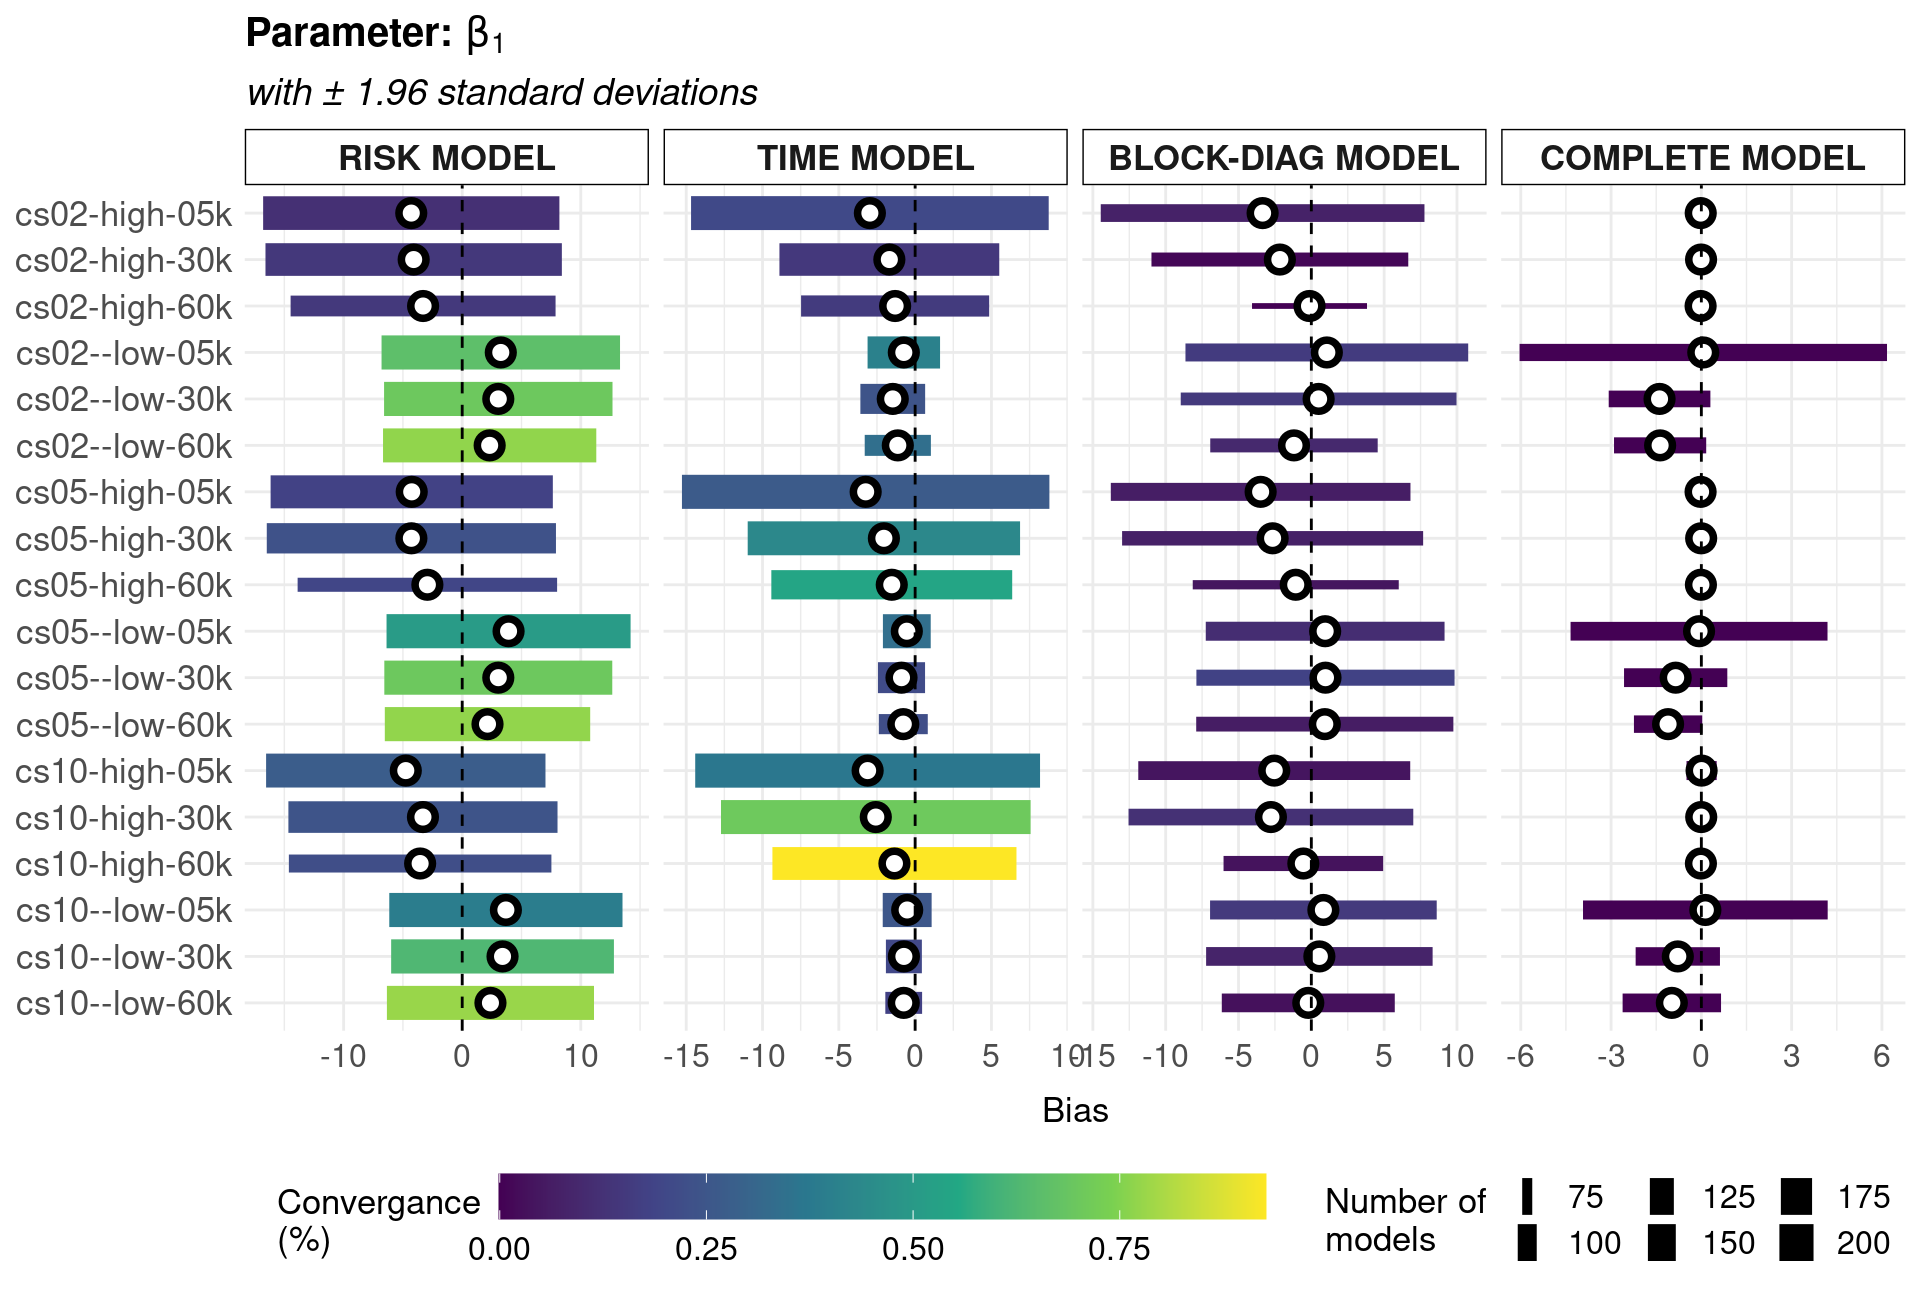
\includegraphics[width=\textwidth]{bias2plotsd-1.png}\\
 \begin{footnotesize}
  SOURCE: The author (2021).
 \end{footnotesize}
 \label{fig:biassdbeta1}
\end{figure}

\begin{figure}[H]
 \setlength{\abovecaptionskip}{.0001pt}
 \caption{PARAMETER \(\beta_{2}\) BIAS WITH \(\pm\) 1.96 STANDARD
         DEVIATIONS}
 \vspace{0.2cm}\centering
 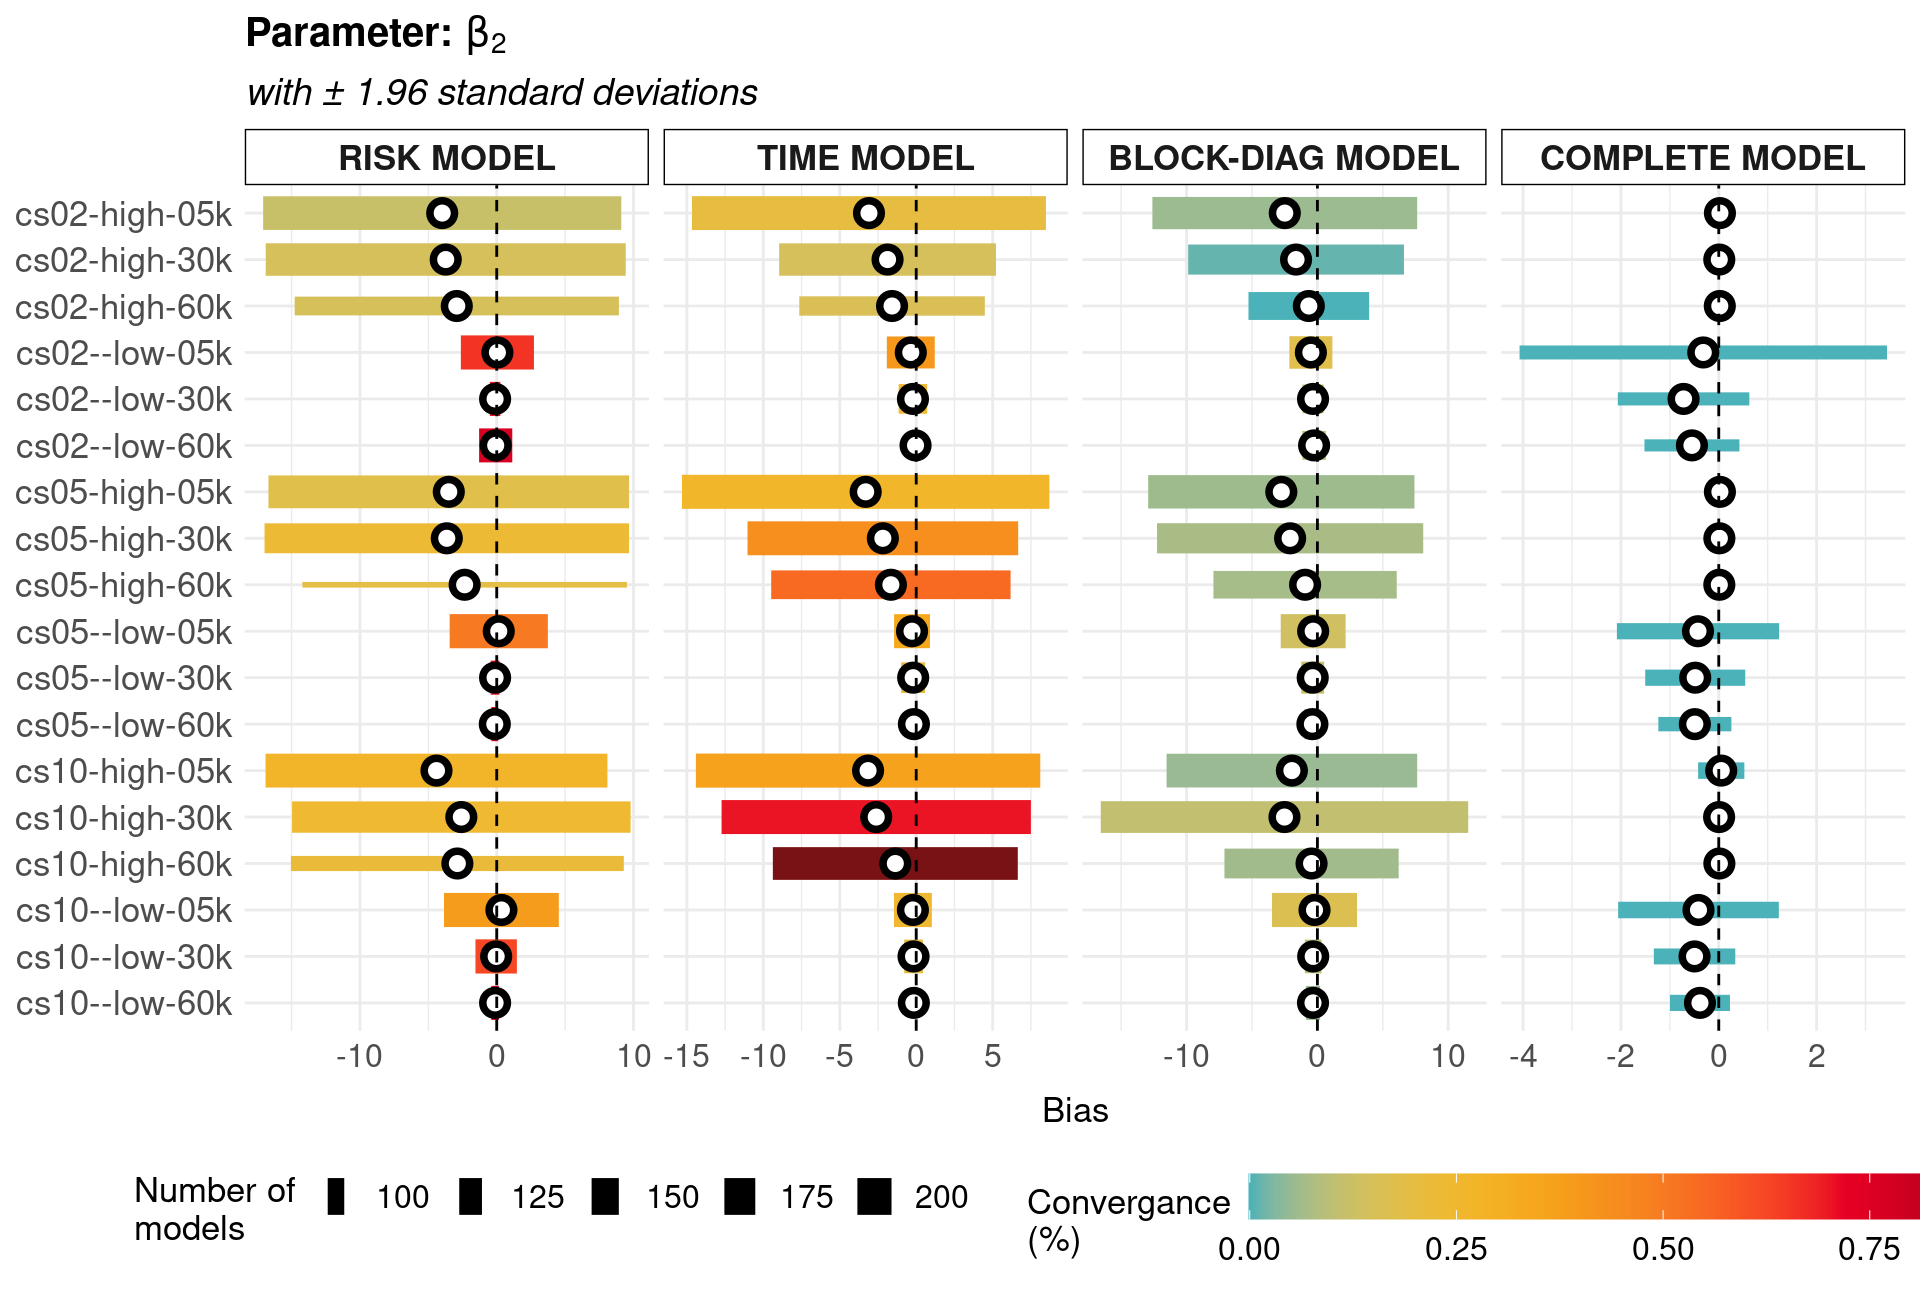
\includegraphics[width=\textwidth]{bias2plotsd-2.png}\\
 \begin{footnotesize}
  SOURCE: The author (2021).
 \end{footnotesize}
 \label{fig:biassdbeta2}
\end{figure}

\begin{figure}[H]
 \setlength{\abovecaptionskip}{.0001pt}
 \caption{PARAMETER \(\gamma_{1}\) BIAS WITH \(\pm\) 1.96 STANDARD
          DEVIATIONS}
 \vspace{0.2cm}\centering
 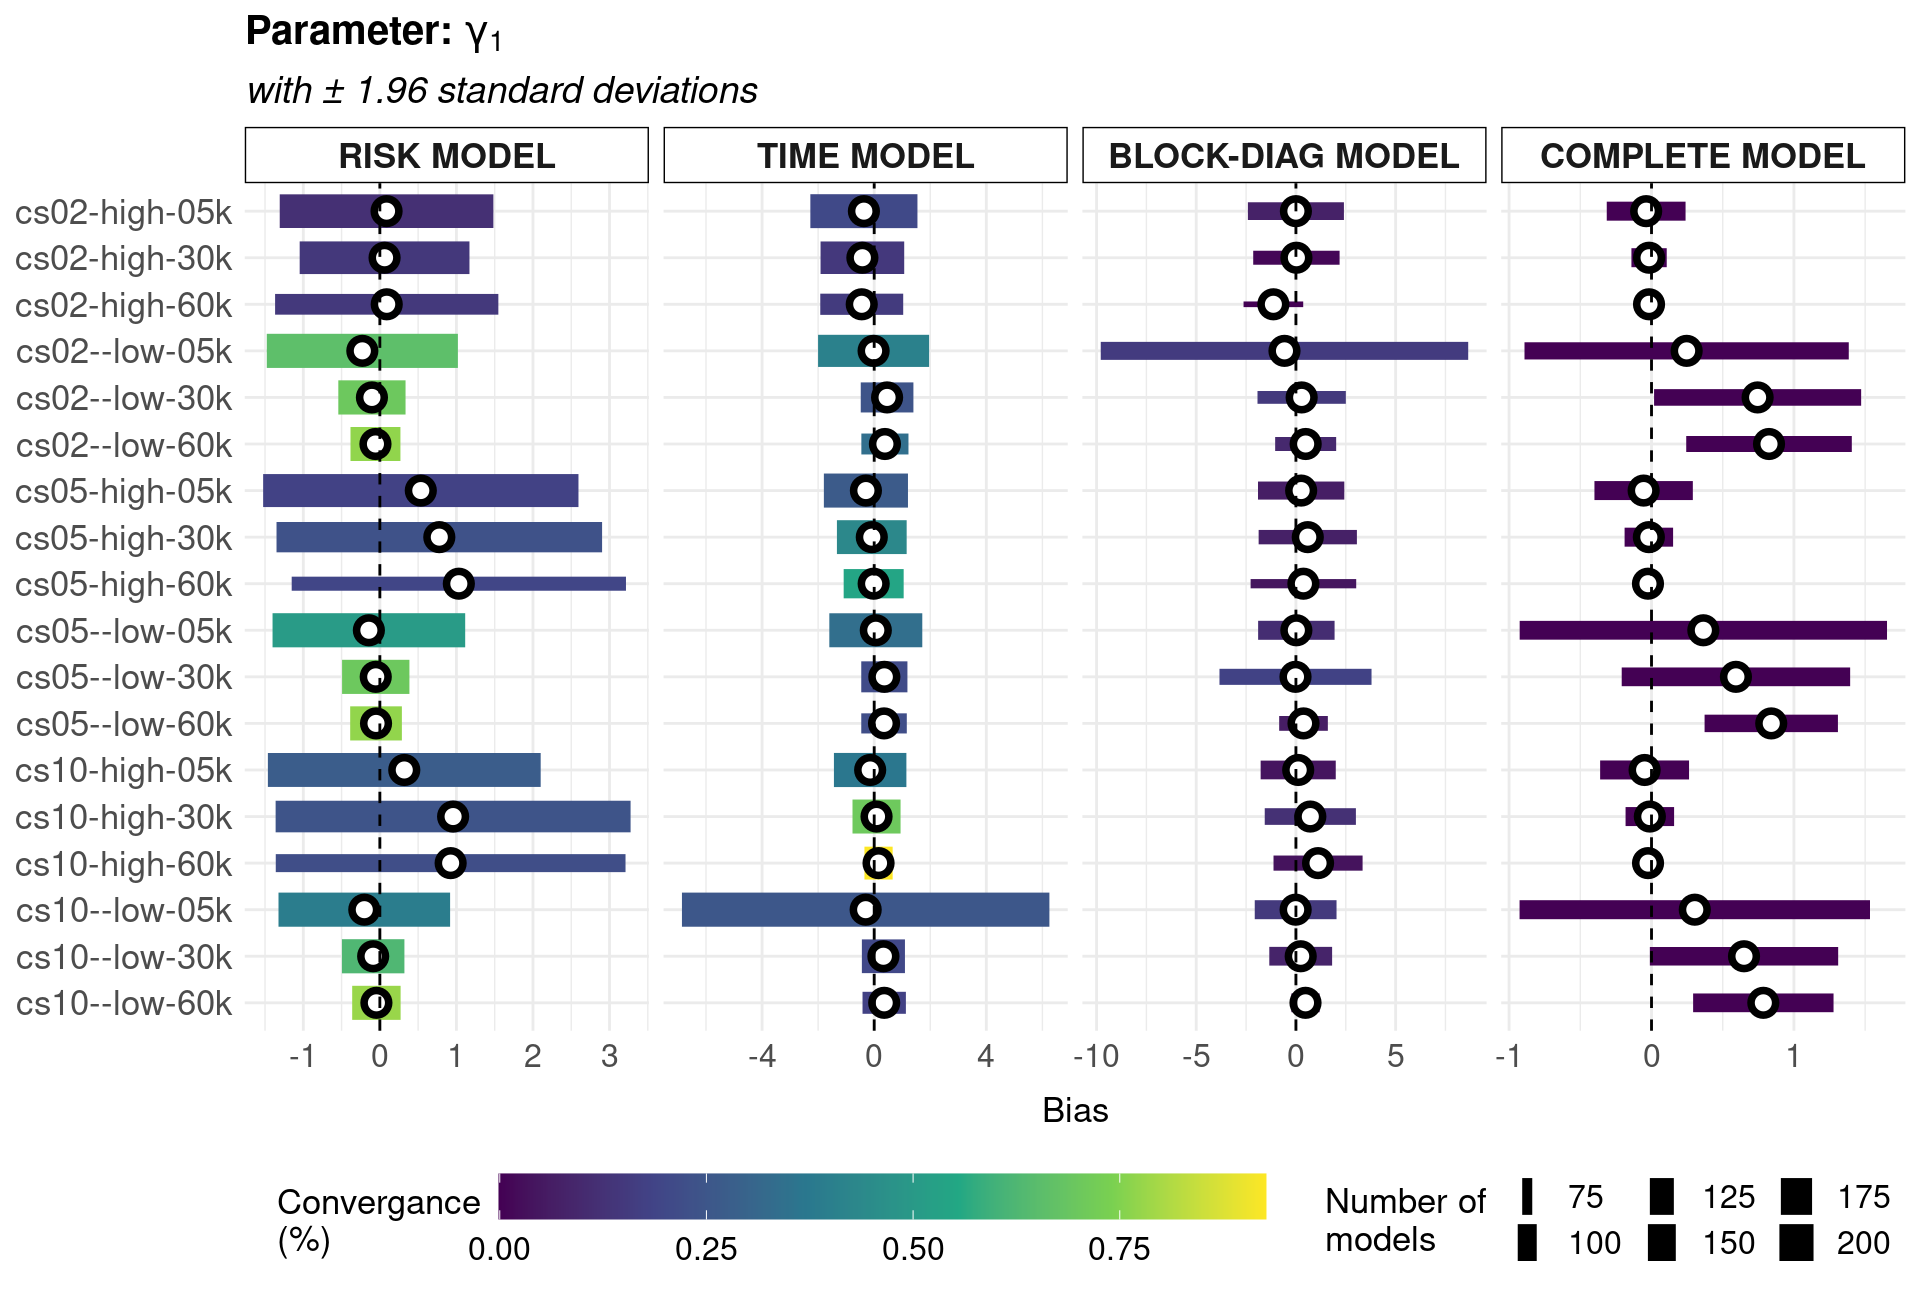
\includegraphics[width=\textwidth]{bias2plotsd-3.png}\\
 \begin{footnotesize}
  SOURCE: The author (2021).
 \end{footnotesize}
 \label{fig:biassdgama1}
\end{figure}

\begin{figure}[H]
 \setlength{\abovecaptionskip}{.0001pt}
 \caption{PARAMETER \(\gamma_{2}\) BIAS WITH \(\pm\) 1.96 STANDARD
          DEVIATIONS}
 \vspace{0.2cm}\centering
 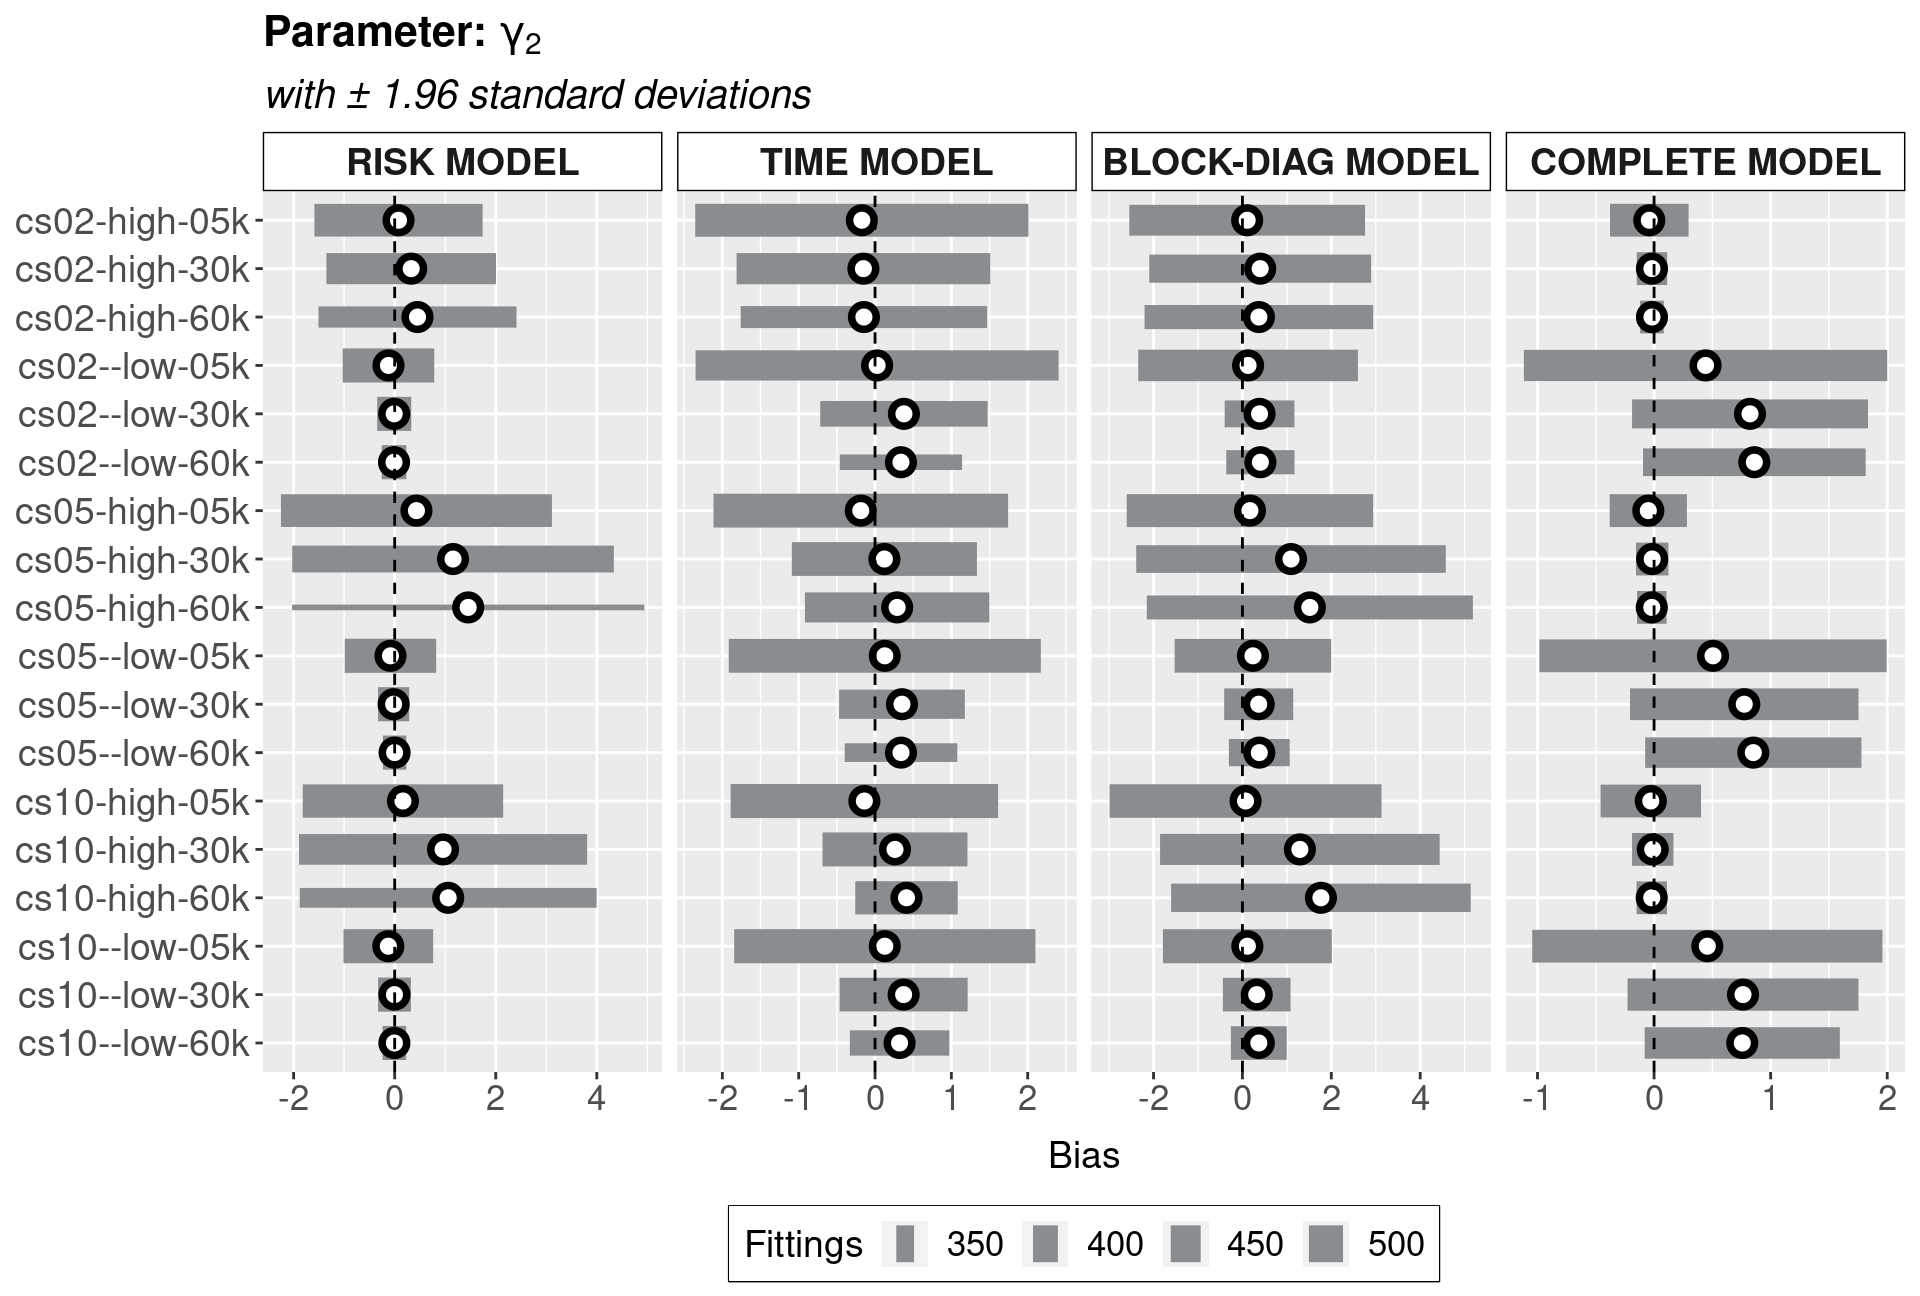
\includegraphics[width=\textwidth]{bias2plotsd-4.png}\\
 \begin{footnotesize}
  SOURCE: The author (2021).
 \end{footnotesize}
 \label{fig:biassdgama2}
\end{figure}

\begin{figure}[H]
 \setlength{\abovecaptionskip}{.0001pt}
 \caption{PARAMETER \(w_{1}\) BIAS WITH \(\pm\) 1.96 STANDARD DEVIATIONS}
 \vspace{0.2cm}\centering
 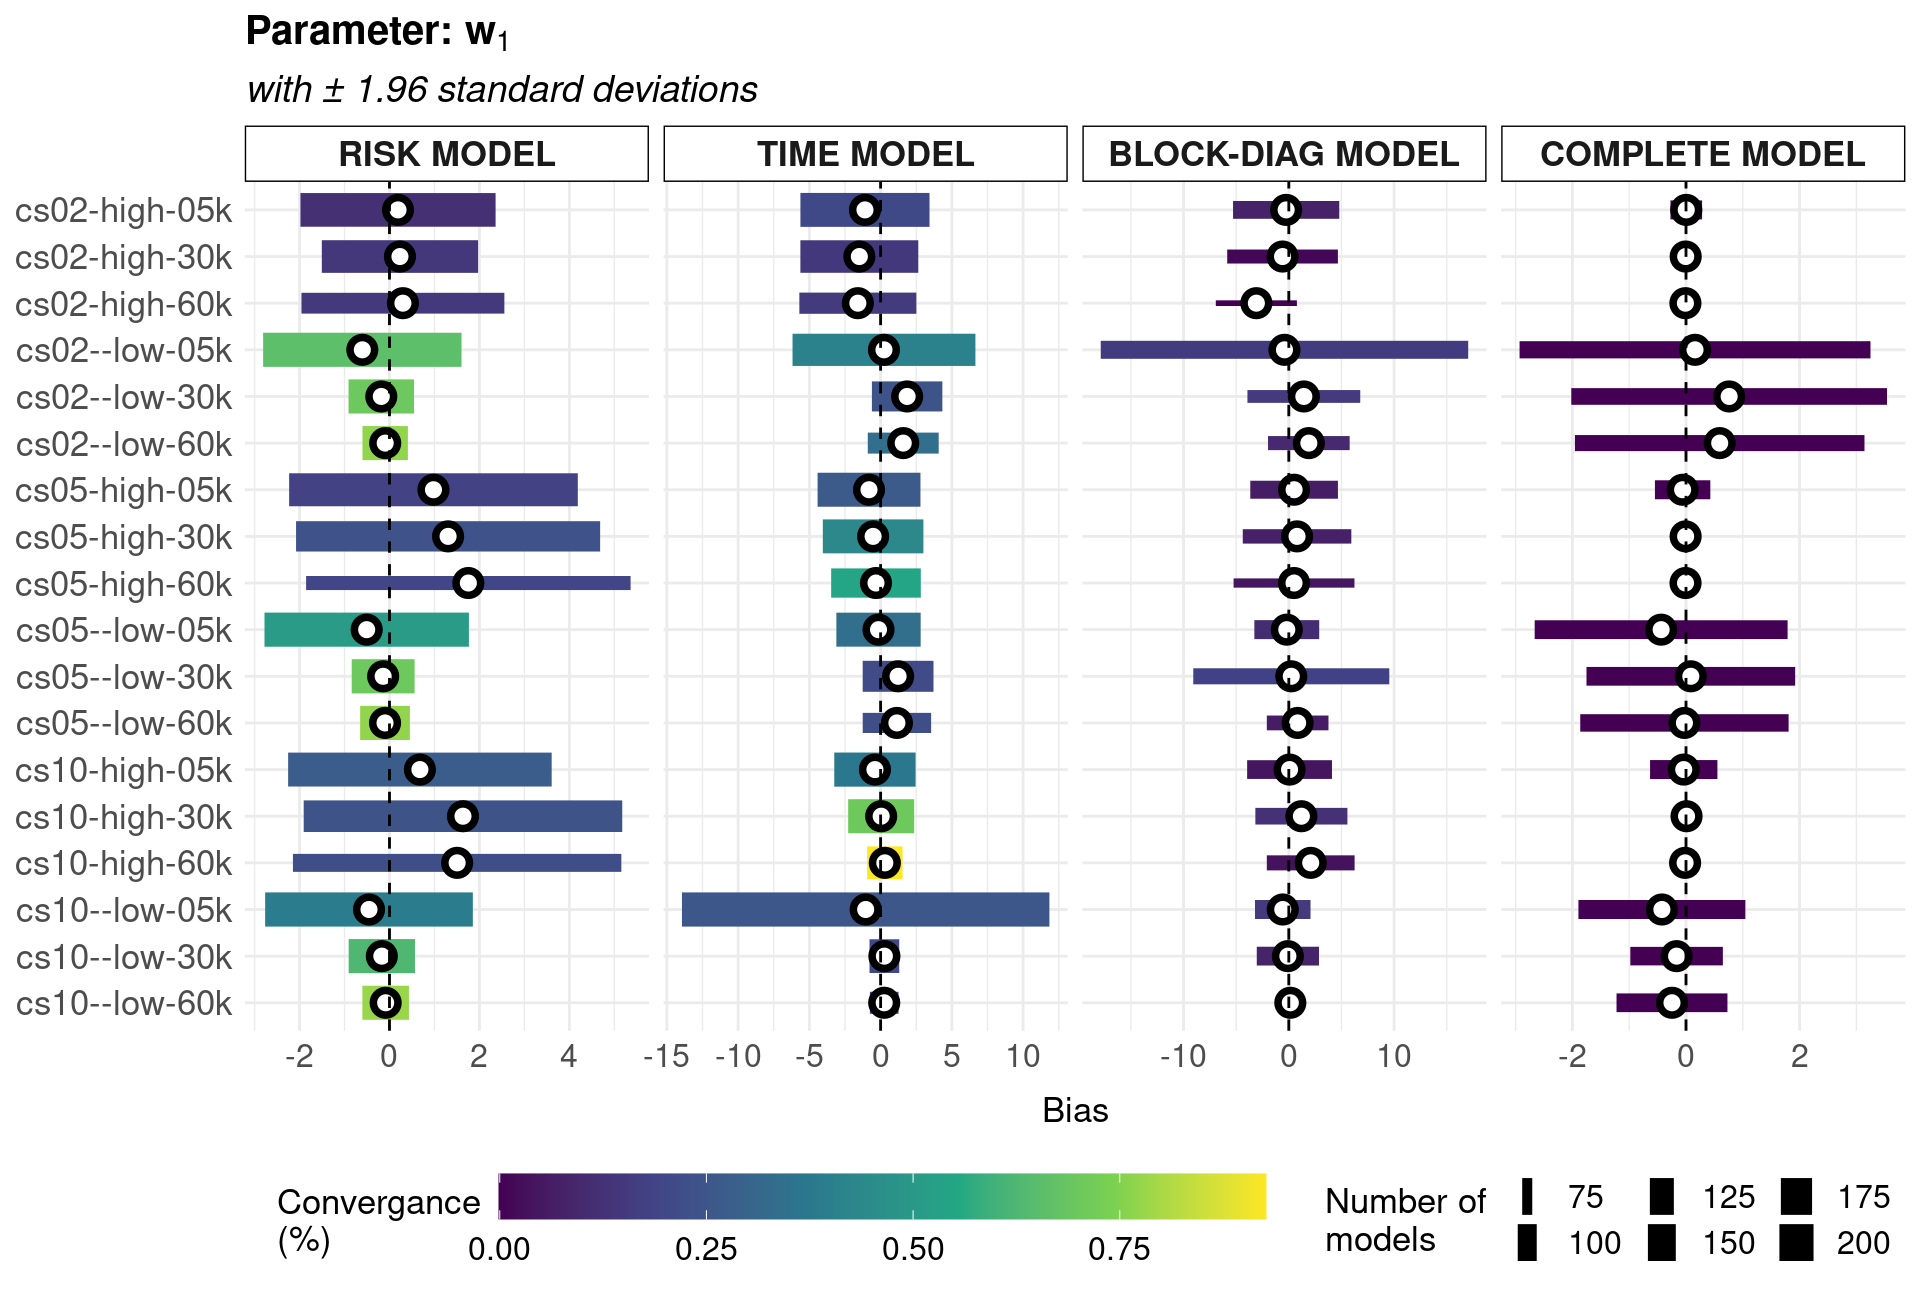
\includegraphics[width=\textwidth]{bias2plotsd-5.png}\\
 \begin{footnotesize}
  SOURCE: The author (2021).
 \end{footnotesize}
 \label{fig:biassdw1}
\end{figure}

\begin{figure}[H]
 \setlength{\abovecaptionskip}{.0001pt}
 \caption{PARAMETER \(w_{2}\) BIAS WITH \(\pm\) 1.96 STANDARD DEVIATIONS}
 \vspace{0.2cm}\centering
 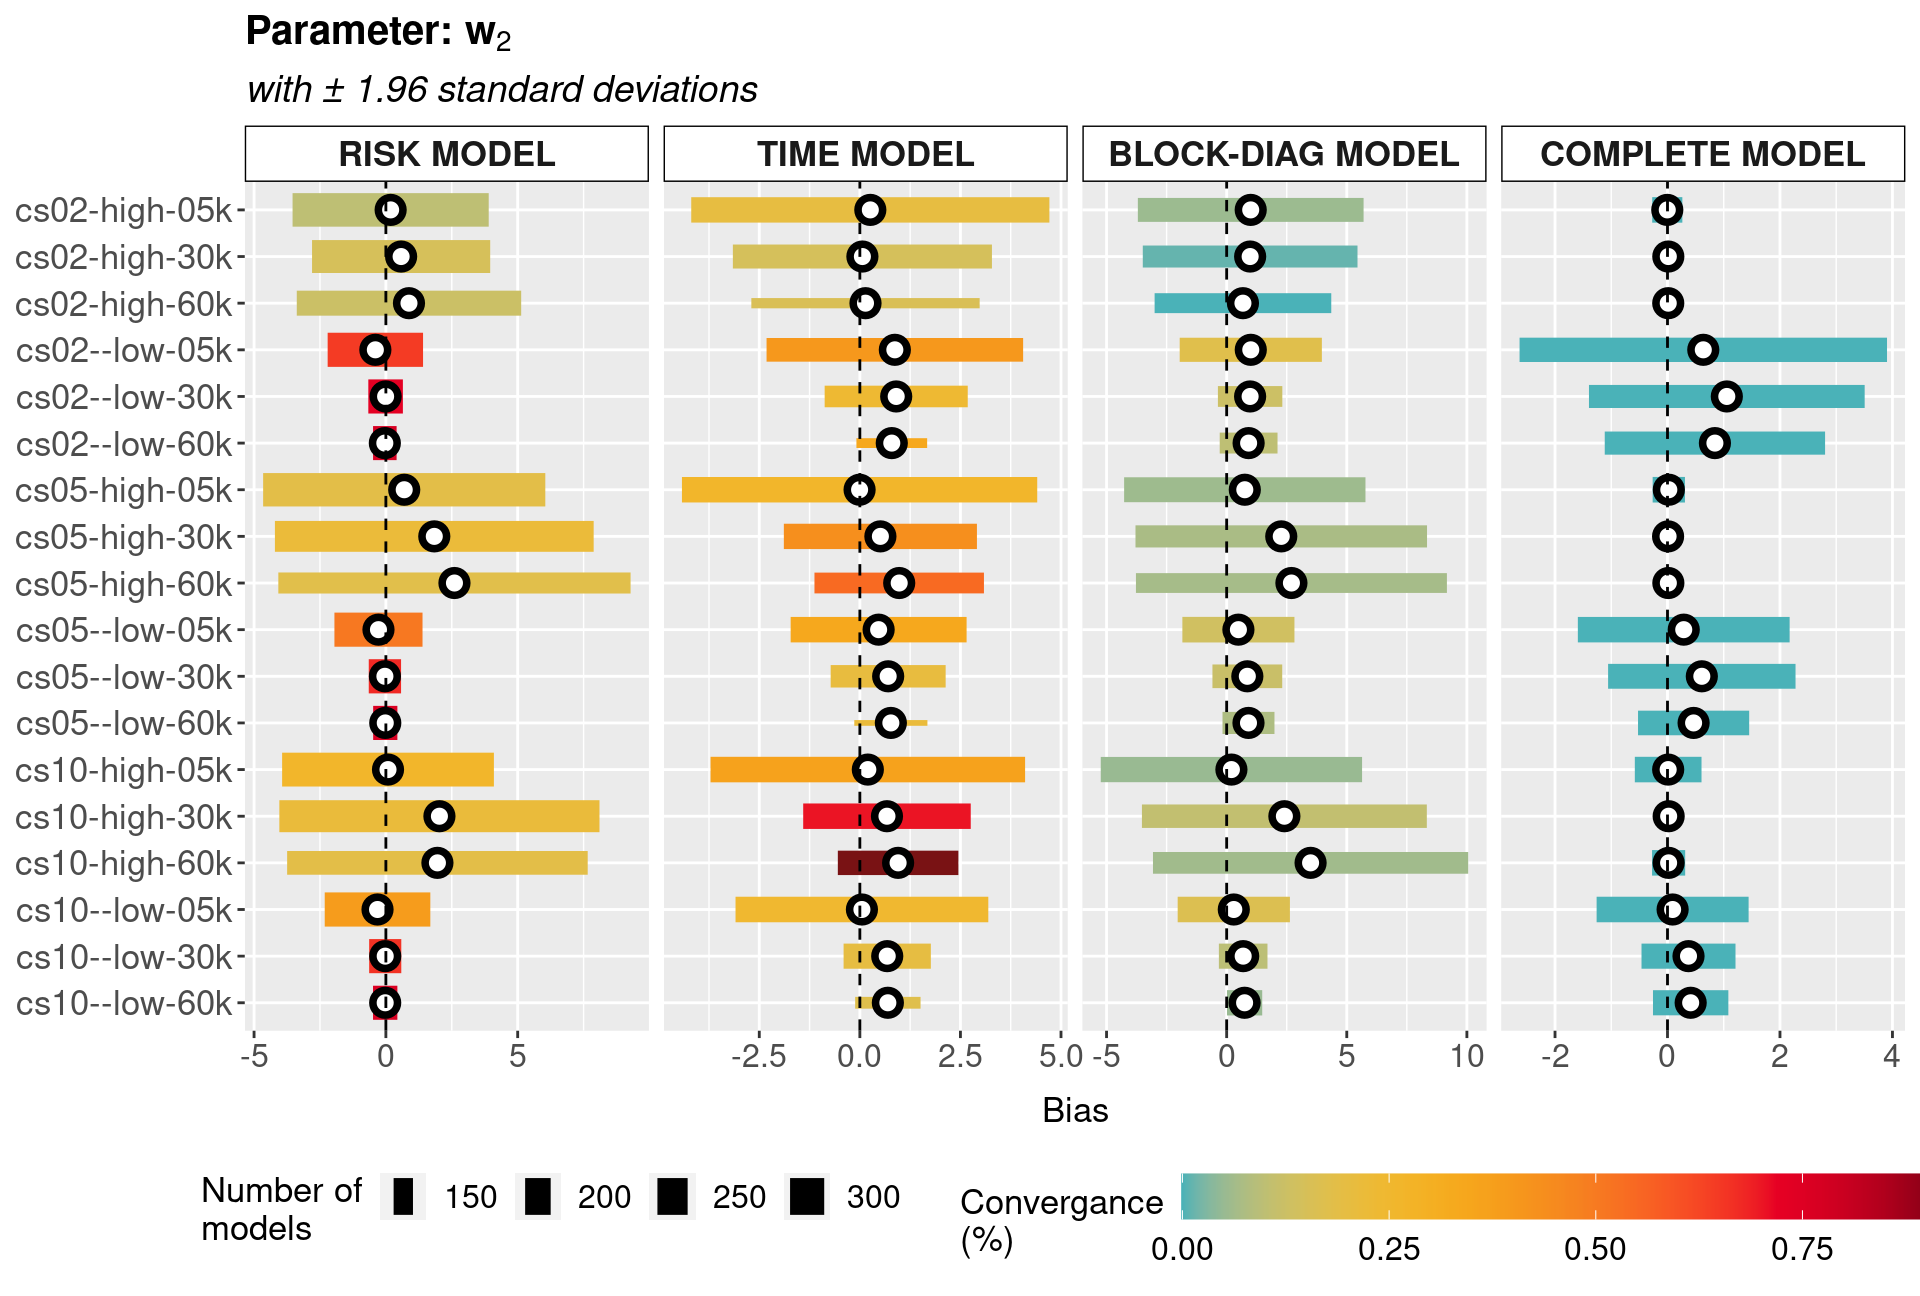
\includegraphics[width=\textwidth]{bias2plotsd-6.png}\\
 \begin{footnotesize}
  SOURCE: The author (2021).
 \end{footnotesize}
 \label{fig:biassdw2}
\end{figure}

\begin{figure}[H]
 \setlength{\abovecaptionskip}{.0001pt}
 \caption{PARAMETER \(\log(\sigma_{1}^{2})\) BIAS WITH \(\pm\) 1.96
          STANDARD DEVIATIONS}
 \vspace{0.2cm}\centering
 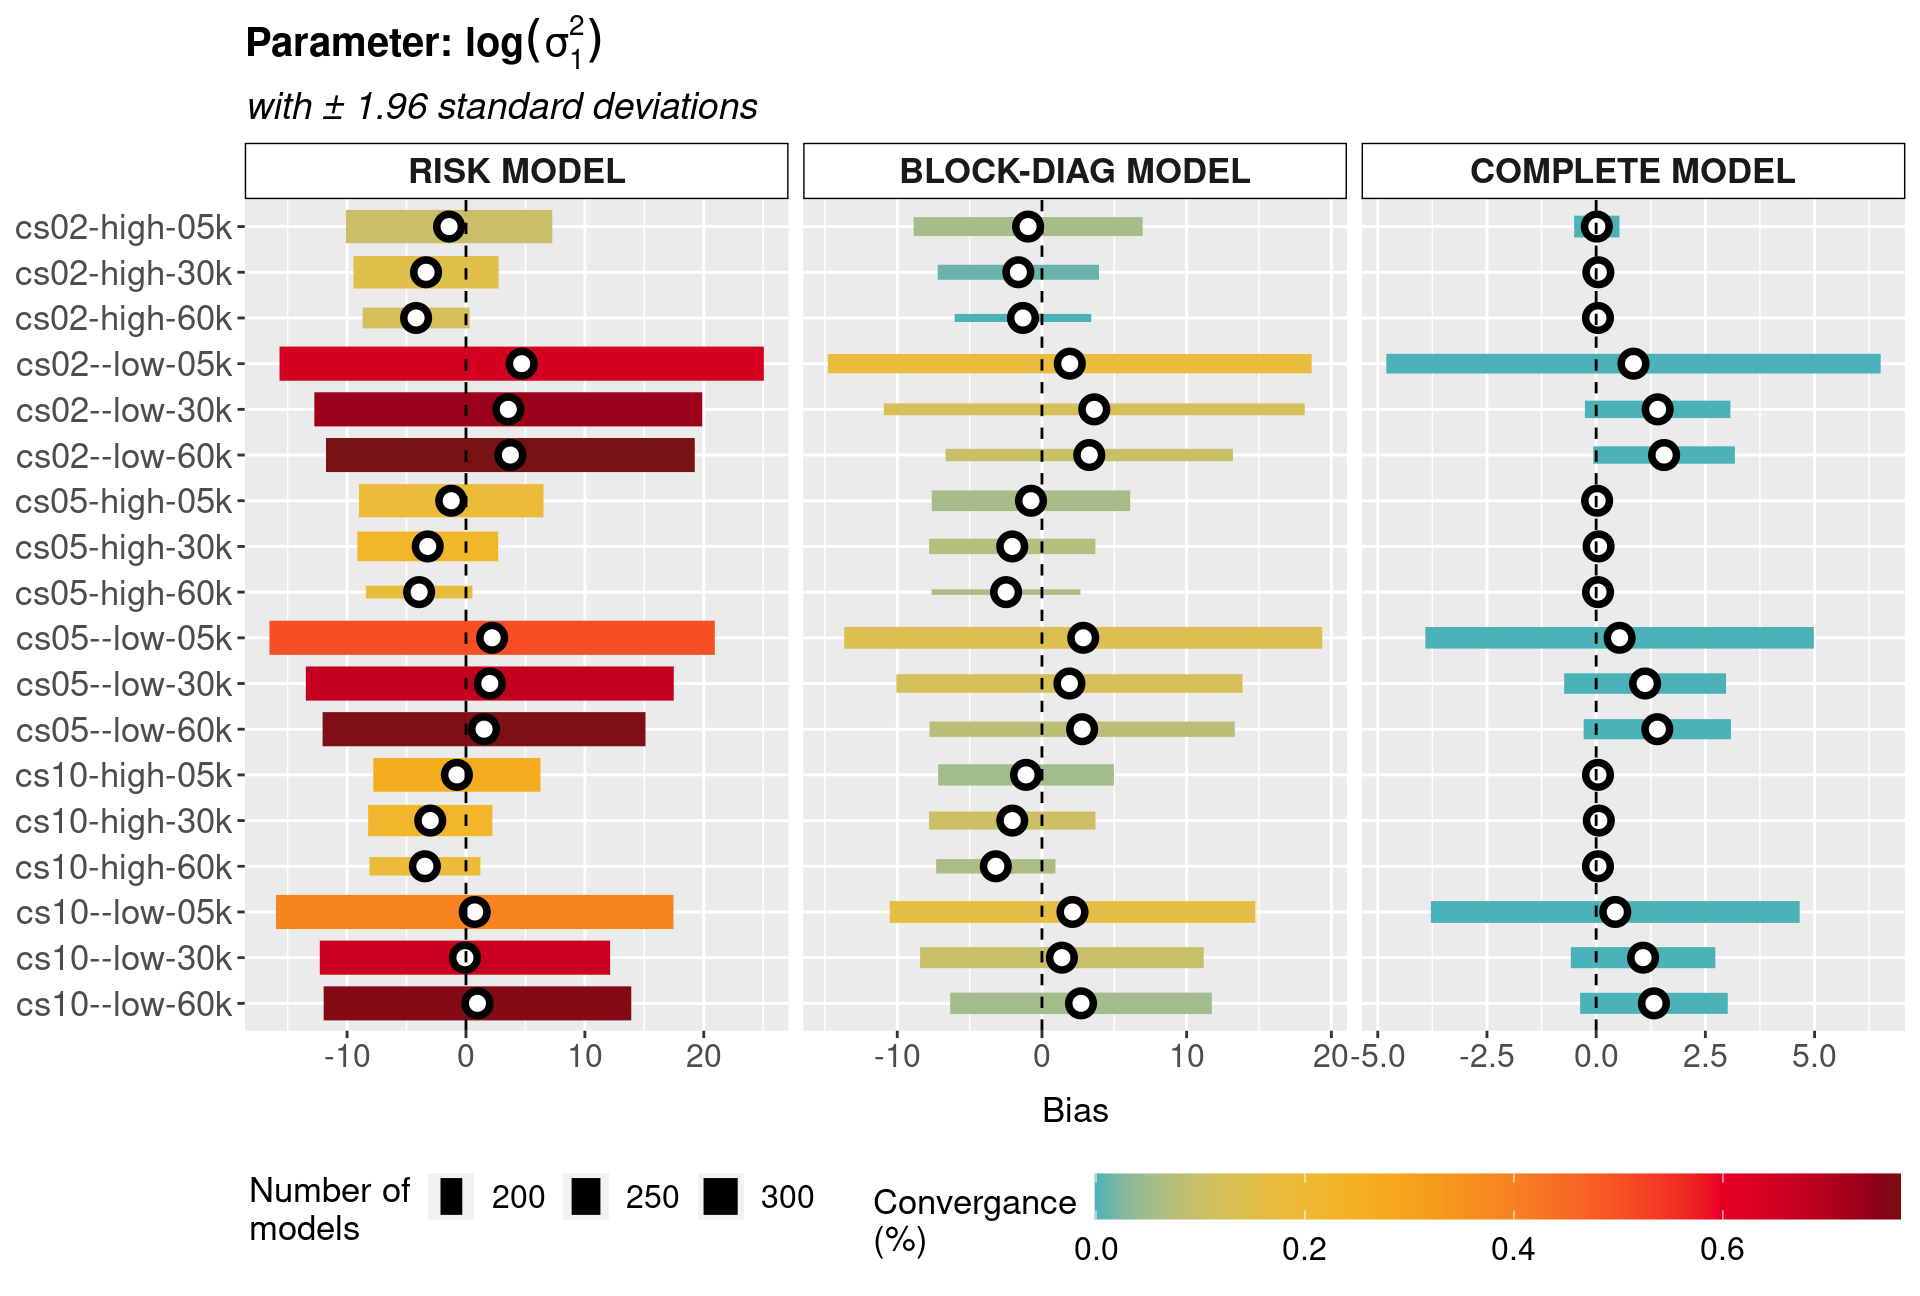
\includegraphics[width=\textwidth]{bias2plotsd-7.png}\\
 \begin{footnotesize}
  SOURCE: The author (2021).
 \end{footnotesize}
 \label{fig:biassdlogs2_1}
\end{figure}

\begin{figure}[H]
 \setlength{\abovecaptionskip}{.0001pt}
 \caption{PARAMETER \(\log(\sigma_{2}^{2})\) BIAS WITH \(\pm\) 1.96
          STANDARD DEVIATIONS}
 \vspace{0.2cm}\centering
 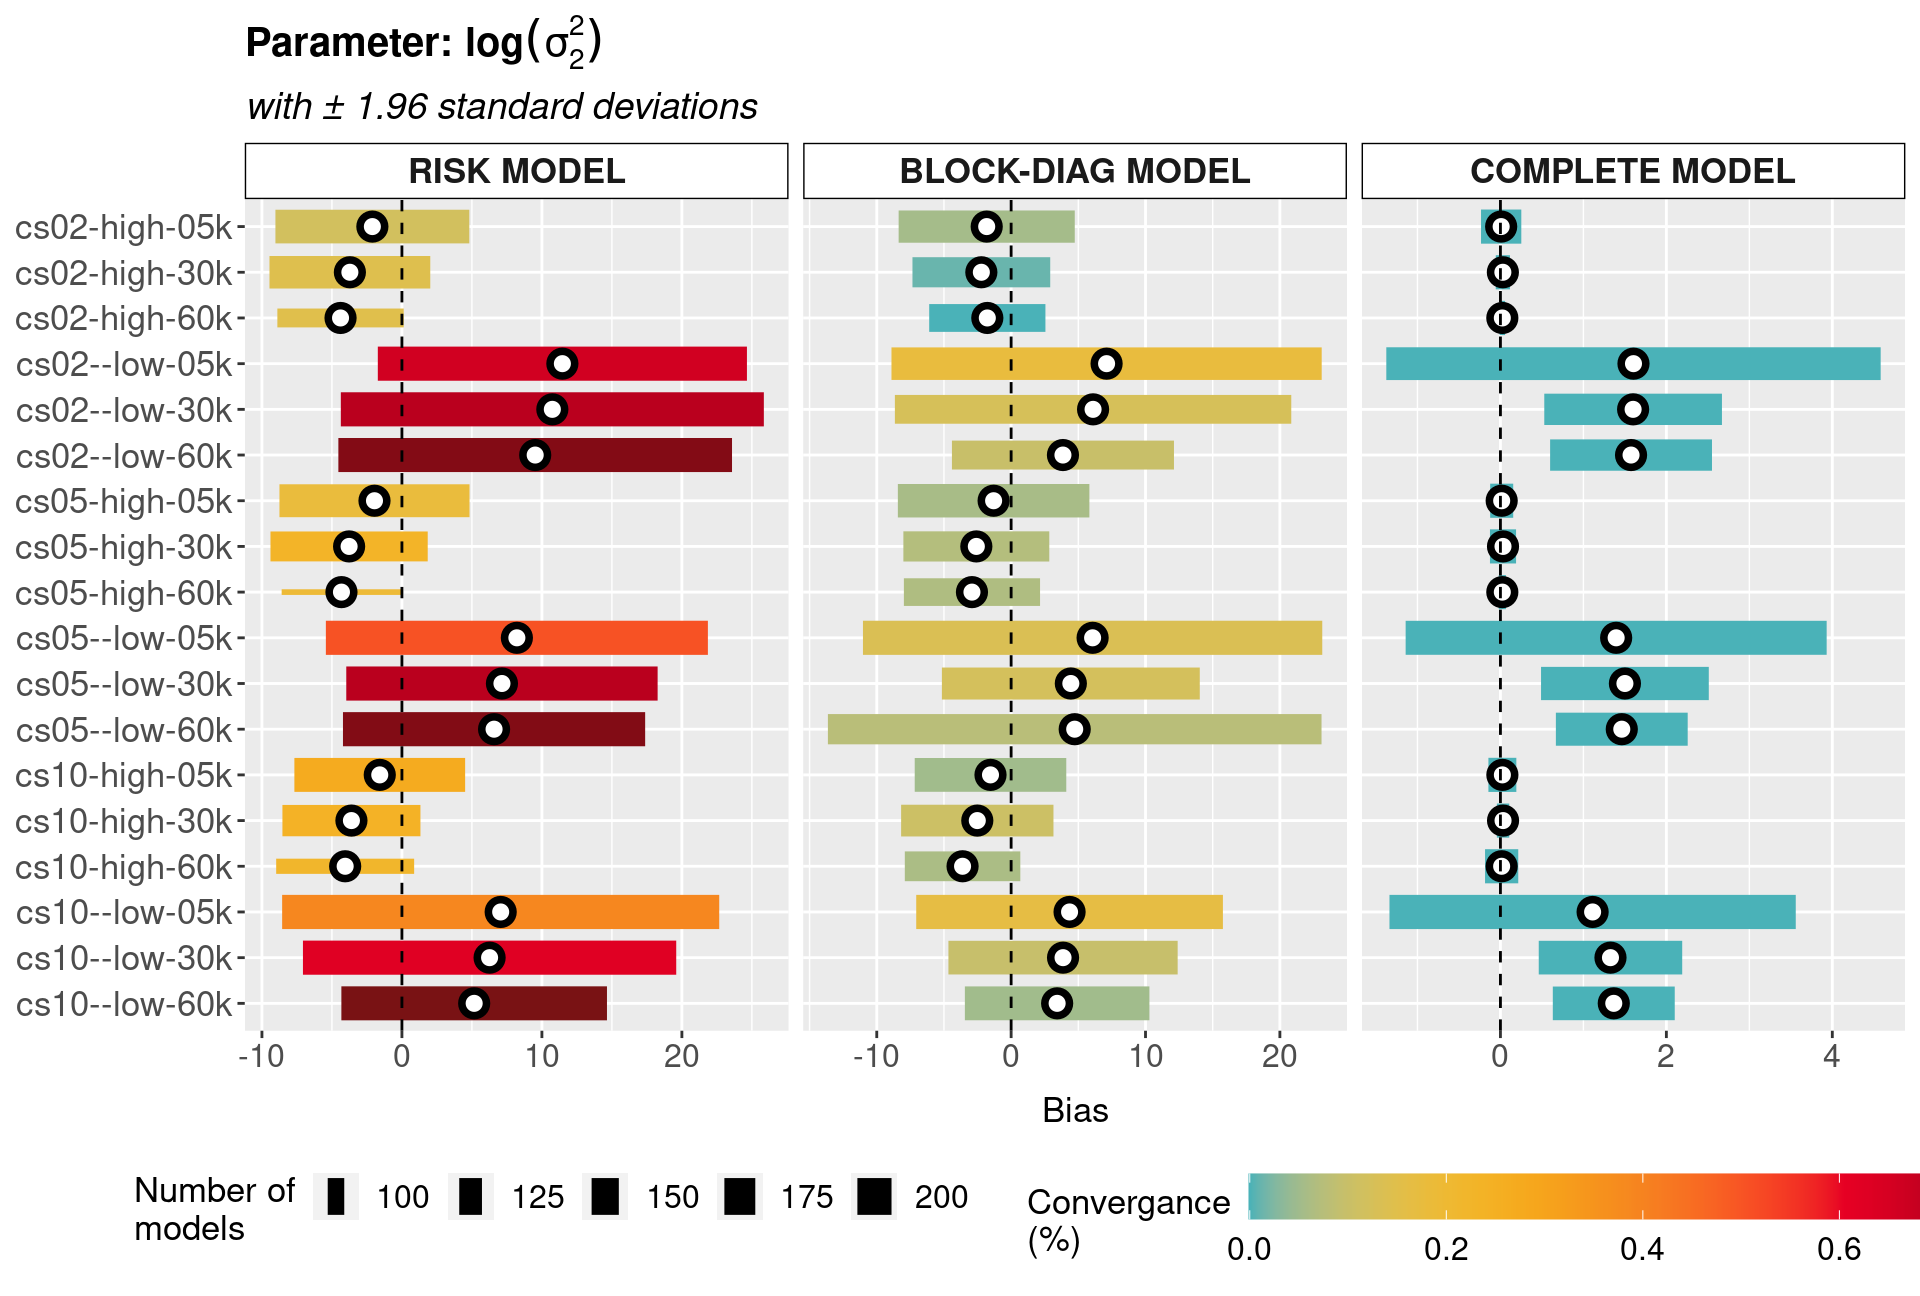
\includegraphics[width=\textwidth]{bias2plotsd-8.png}\\
 \begin{footnotesize}
  SOURCE: The author (2021).
 \end{footnotesize}
 \label{fig:biassdlogs2_2}
\end{figure}

\begin{figure}[H]
 \setlength{\abovecaptionskip}{.0001pt}
 \caption{PARAMETER \(\log(\sigma_{3}^{2})\) BIAS WITH \(\pm\) 1.96
          STANDARD DEVIATIONS}
 \vspace{0.2cm}\centering
 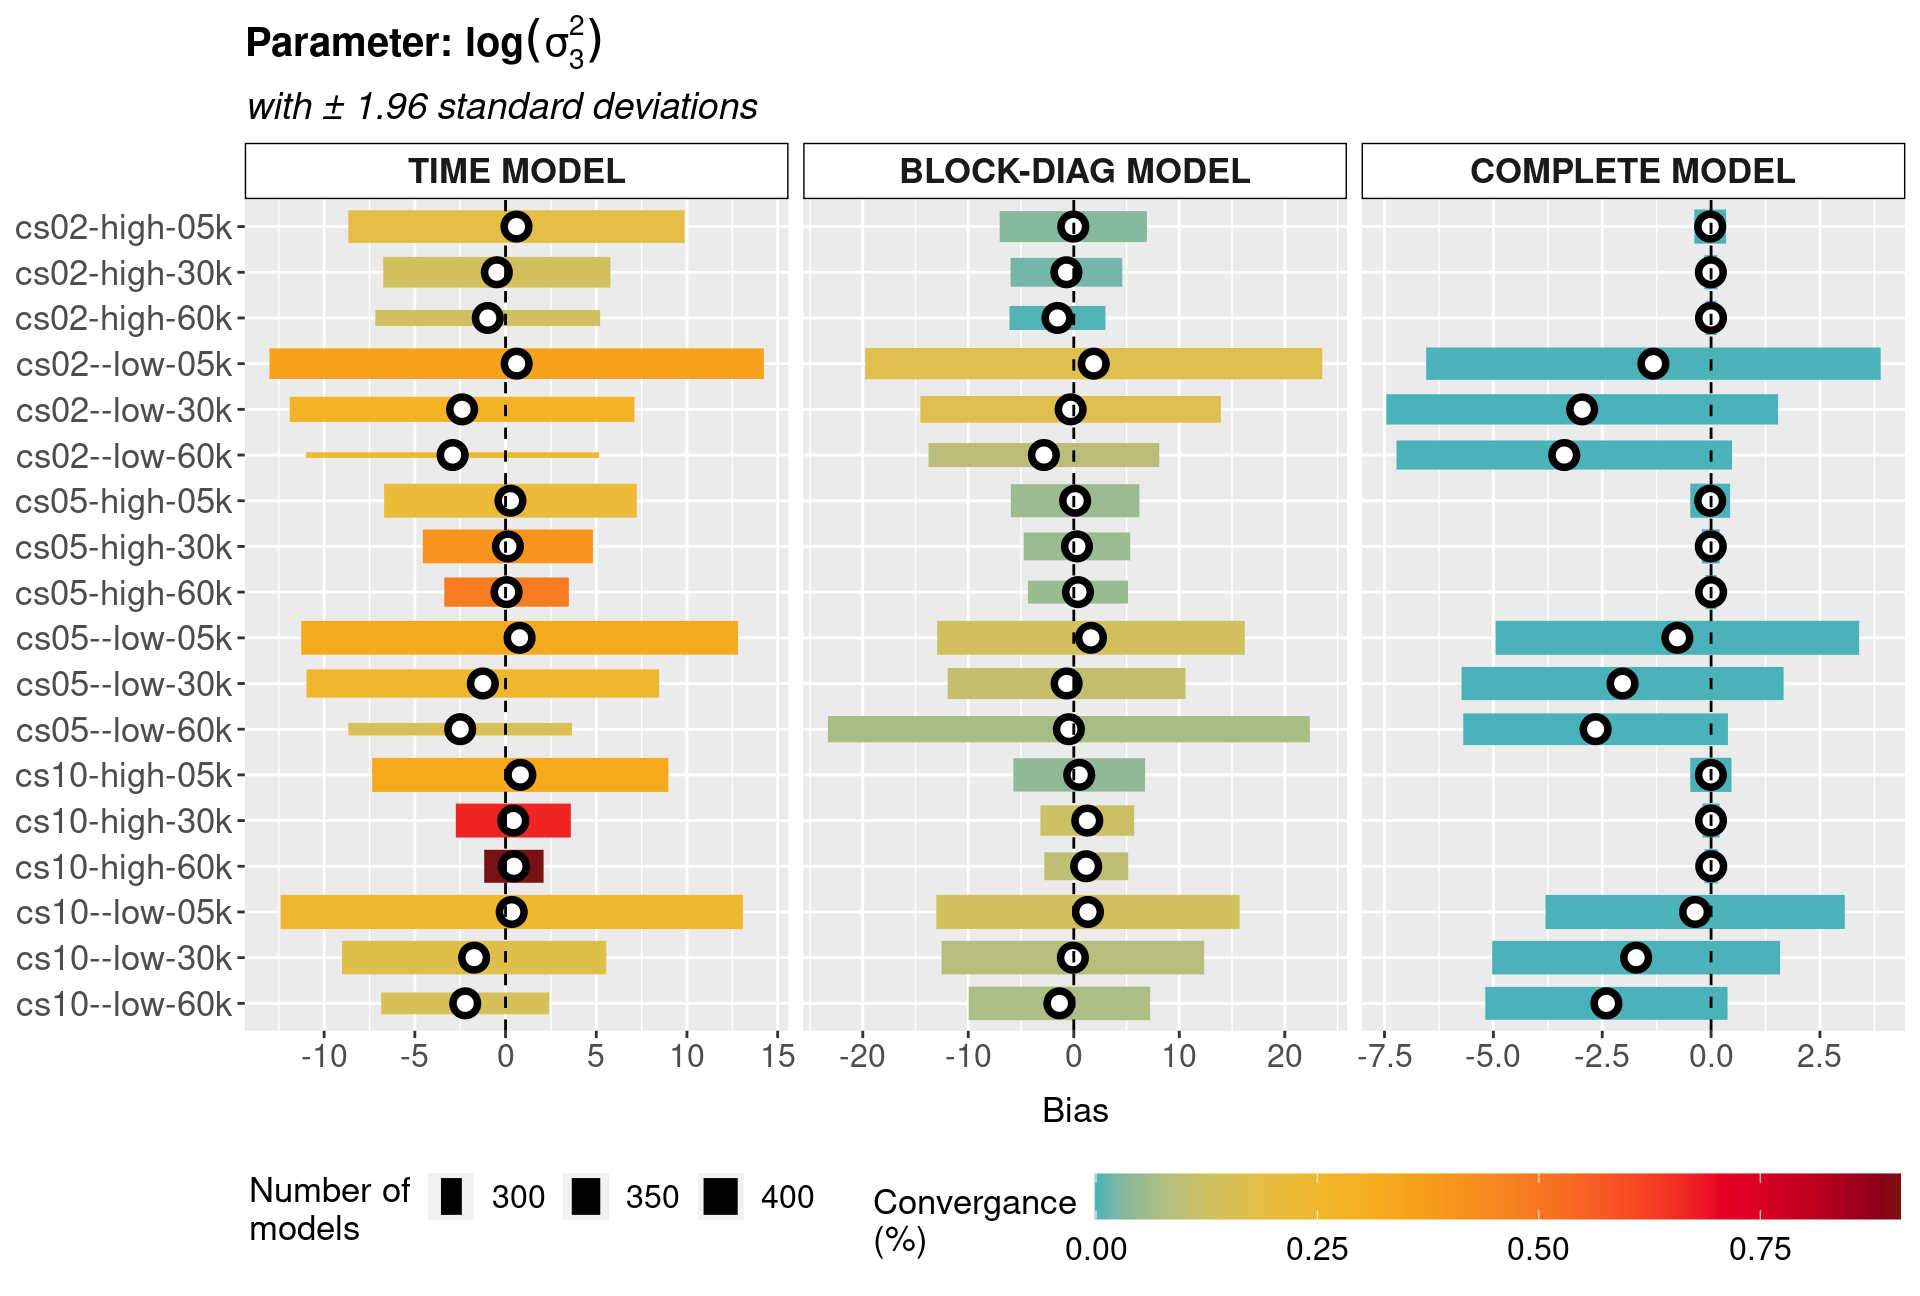
\includegraphics[width=\textwidth]{bias2plotsd-9.png}\\
 \begin{footnotesize}
  SOURCE: The author (2021).
 \end{footnotesize}
 \label{fig:biassdlogs2_3}
\end{figure}

\begin{figure}[H]
 \setlength{\abovecaptionskip}{.0001pt}
 \caption{PARAMETER \(\log(\sigma_{4}^{2})\) BIAS WITH \(\pm\) 1.96
          STANDARD DEVIATIONS}
 \vspace{0.2cm}\centering
 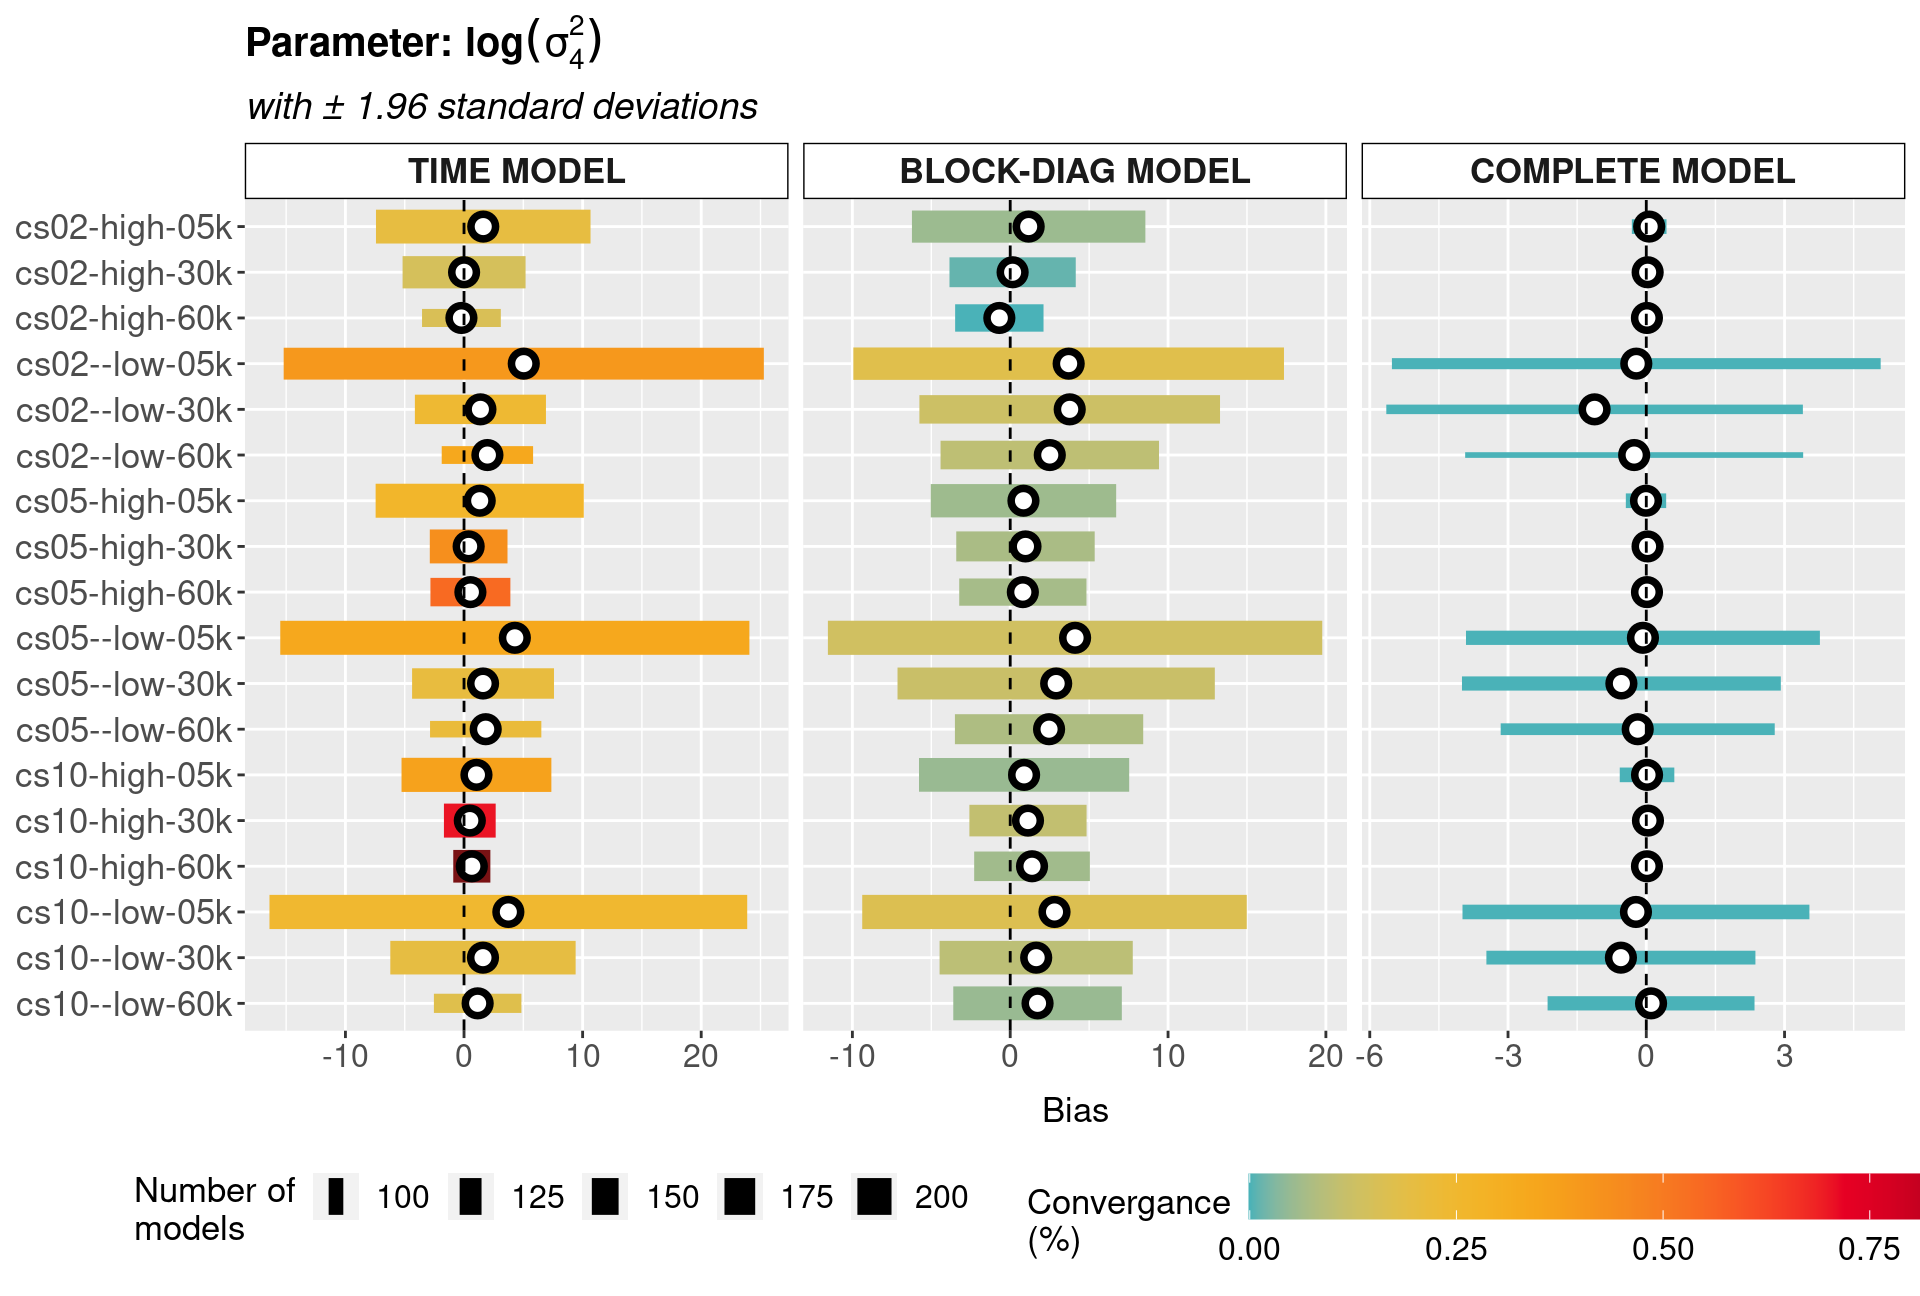
\includegraphics[width=\textwidth]{bias2plotsd-10.png}\\
 \begin{footnotesize}
  SOURCE: The author (2021).
 \end{footnotesize}
 \label{fig:biassdlogs2_4}
\end{figure}

\begin{figure}[H]
 \setlength{\abovecaptionskip}{.0001pt}
 \caption{PARAMETER \(z(\rho_{12})\) BIAS WITH \(\pm\) 1.96 STANDARD
          DEVIATIONS}
 \vspace{0.2cm}\centering
 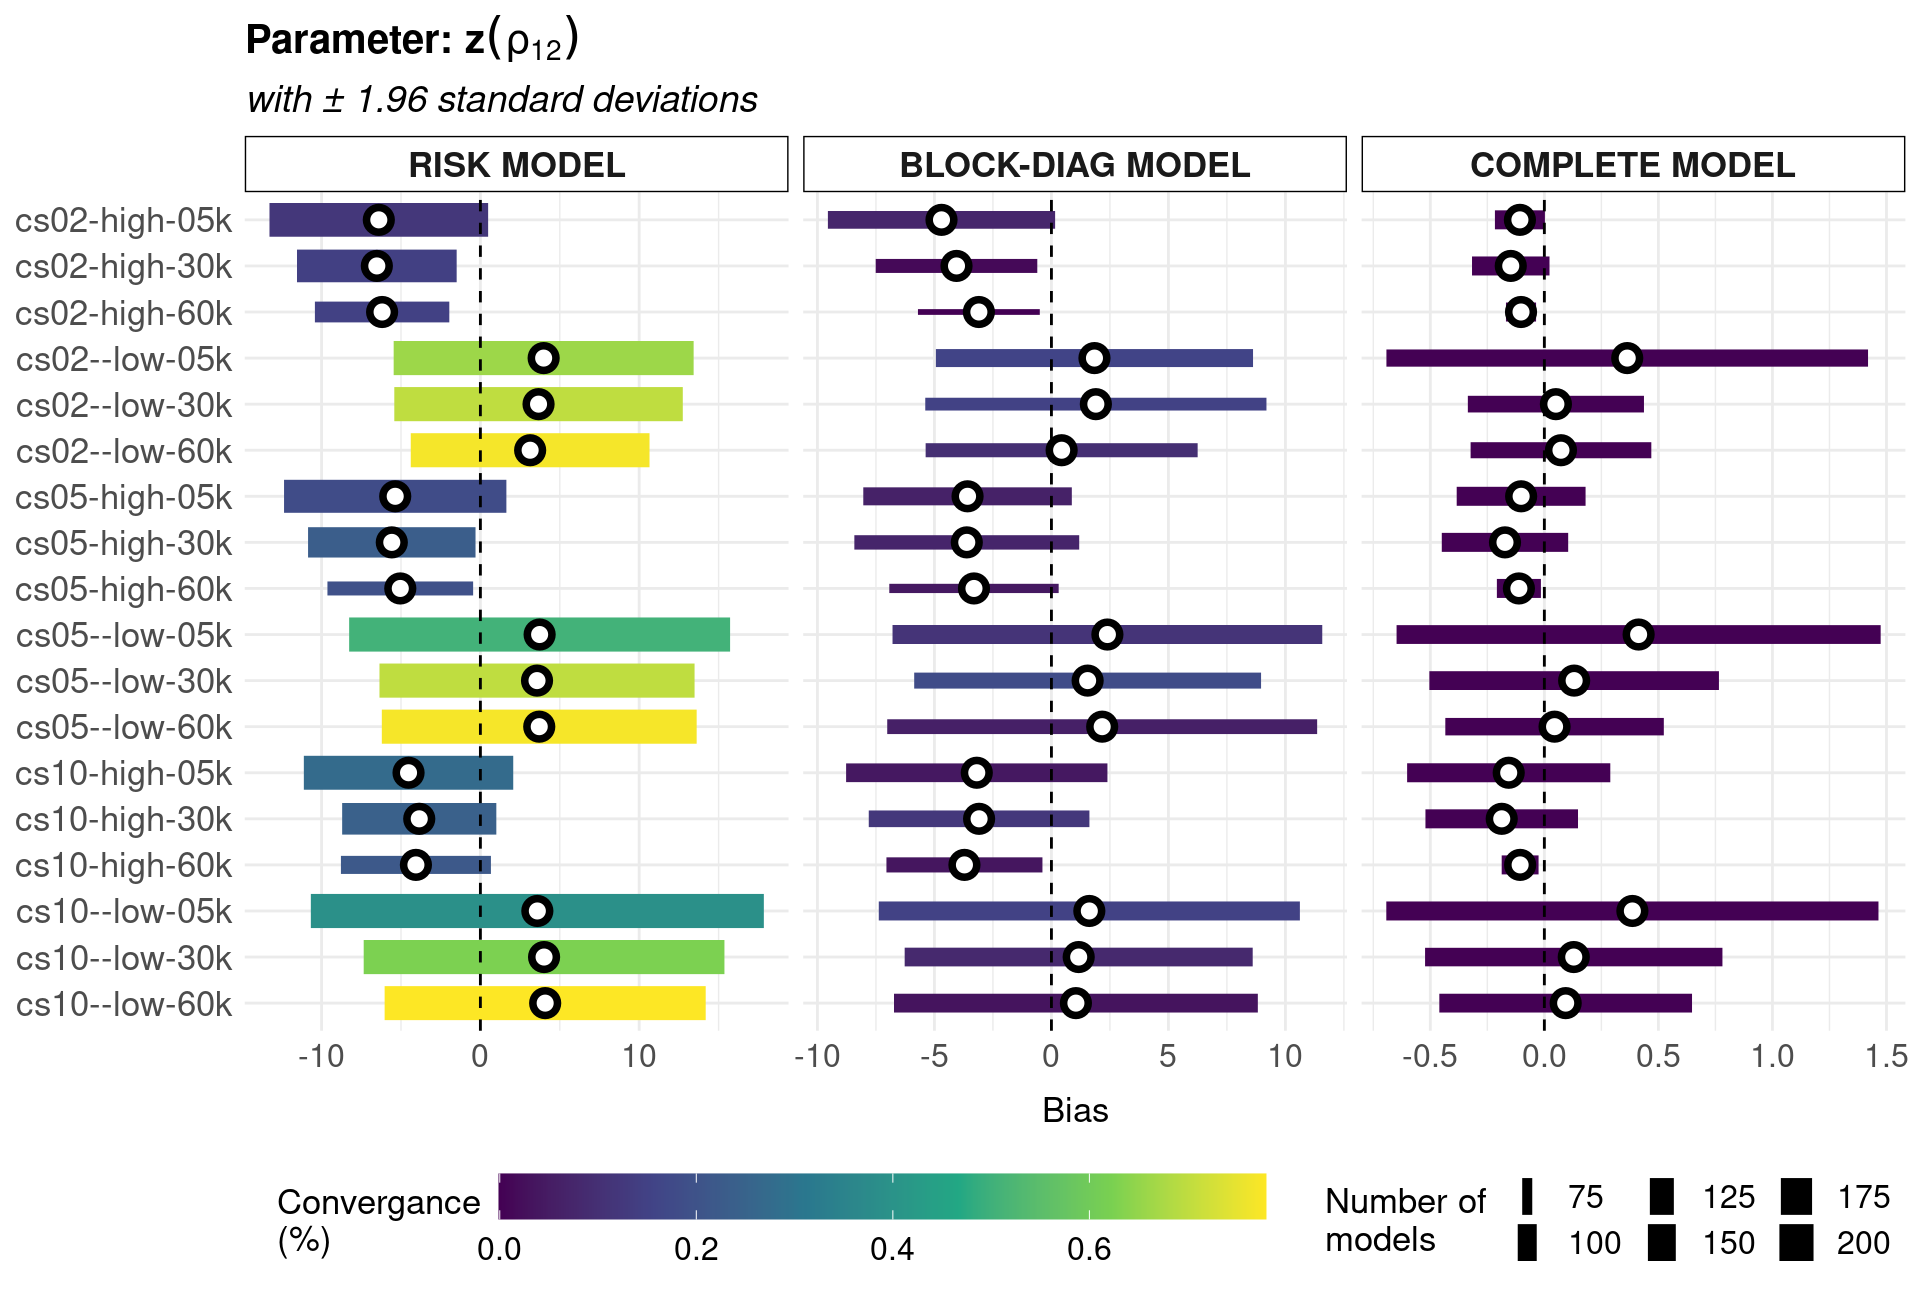
\includegraphics[width=\textwidth]{bias2plotsd-11.png}\\
 \begin{footnotesize}
  SOURCE: The author (2021).
 \end{footnotesize}
 \label{fig:biassdrhoz12}
\end{figure}

\begin{figure}[H]
 \setlength{\abovecaptionskip}{.0001pt}
 \caption{PARAMETER \(z(\rho_{34})\) BIAS WITH \(\pm\) 1.96 STANDARD
          DEVIATIONS}
 \vspace{0.2cm}\centering
 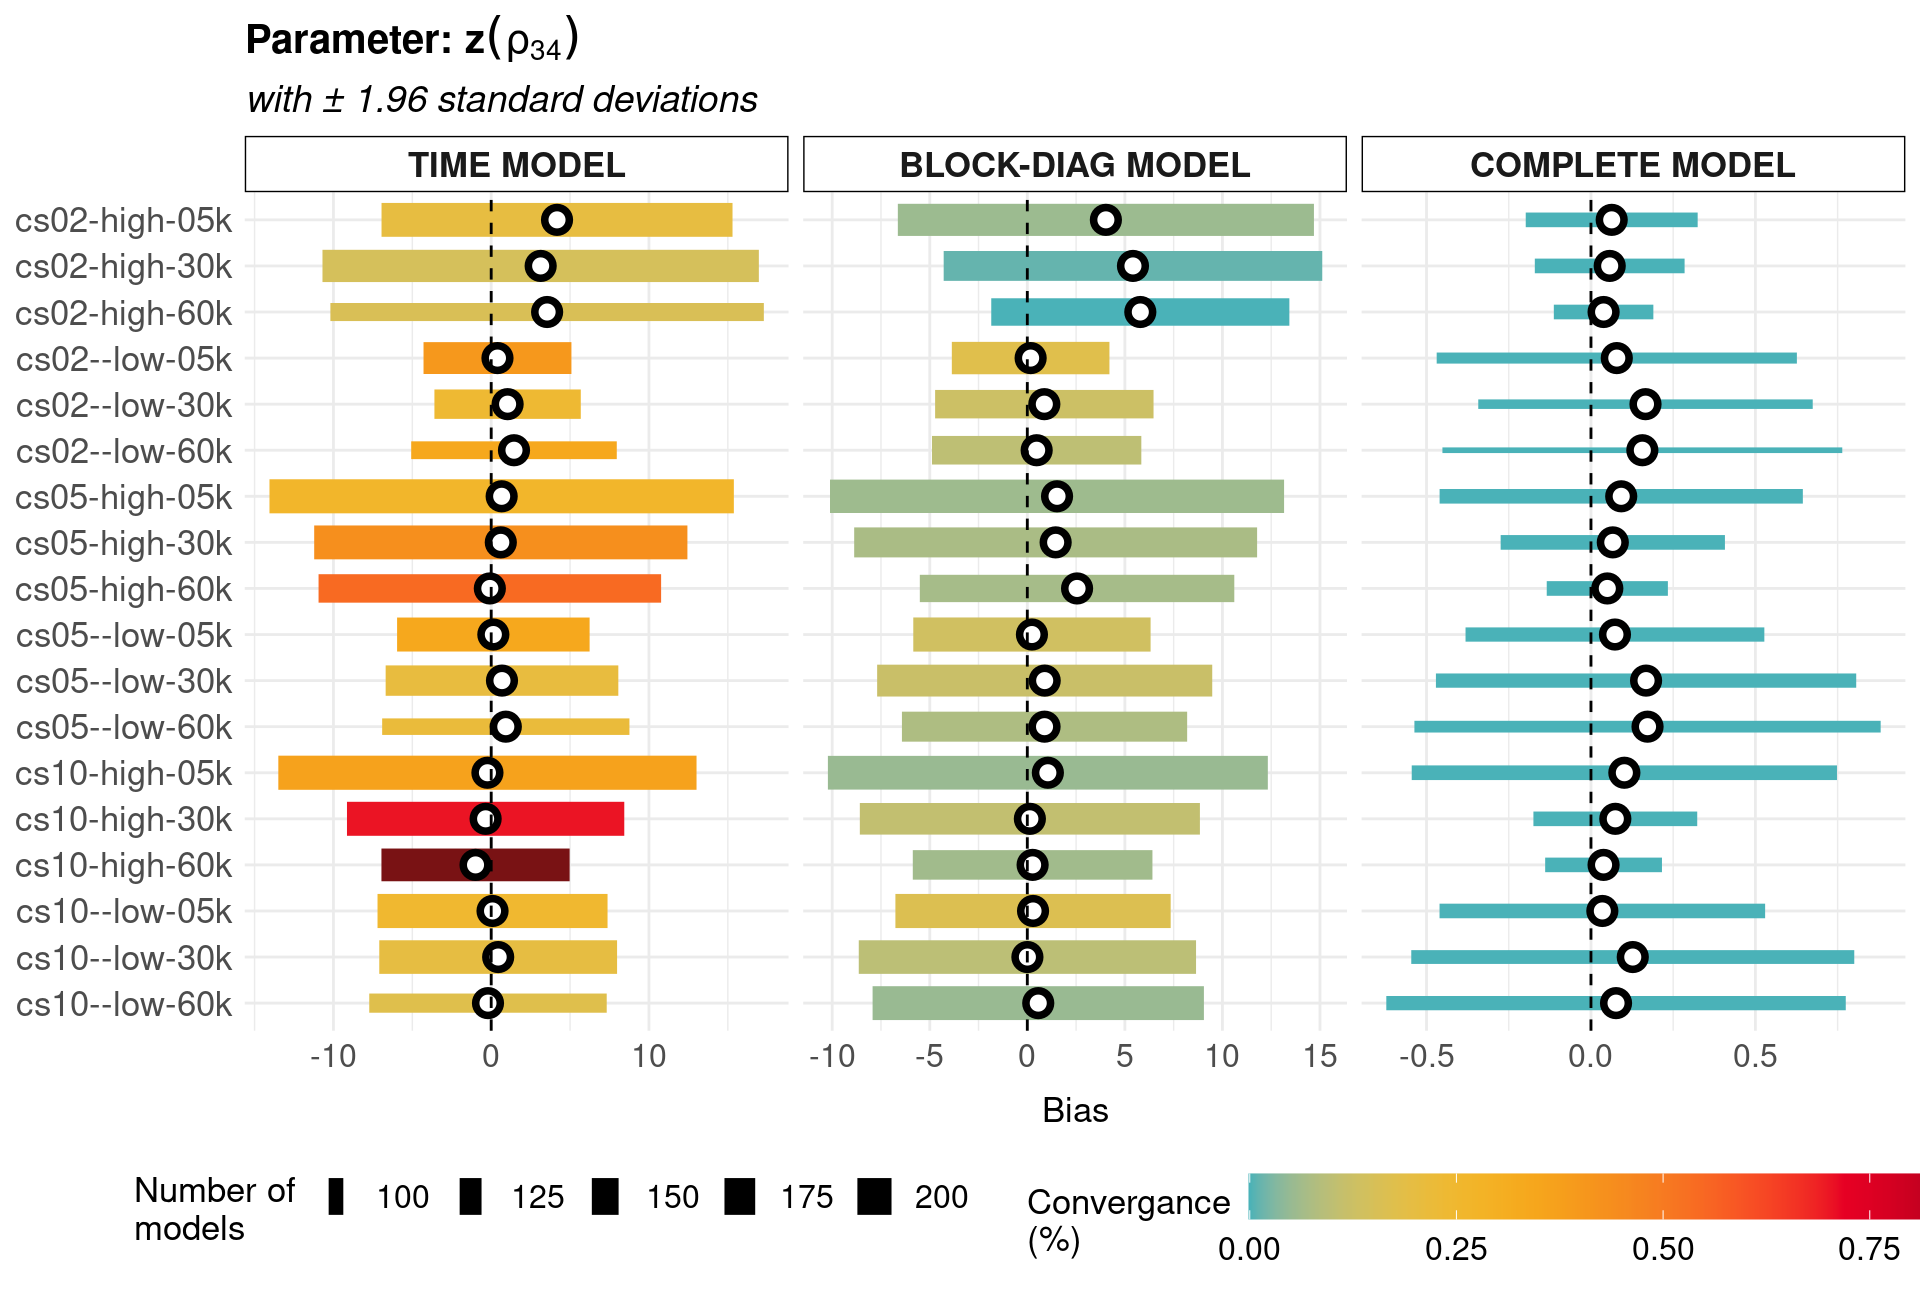
\includegraphics[width=\textwidth]{bias2plotsd-12.png}\\
 \begin{footnotesize}
  SOURCE: The author (2021).
 \end{footnotesize}
 \label{fig:biassdrhoz34}
\end{figure}

\begin{figure}[H]
 \setlength{\abovecaptionskip}{.0001pt}
 \caption{PARAMETERS
          \(\{z(\rho_{13}),~z(\rho_{24}),~z(\rho_{14}),~z(\rho_{23})\}\)
          BIAS WITH \(\pm\) 1.96 STANDARD DEVIATIONS}
 \vspace{0.2cm}\centering
 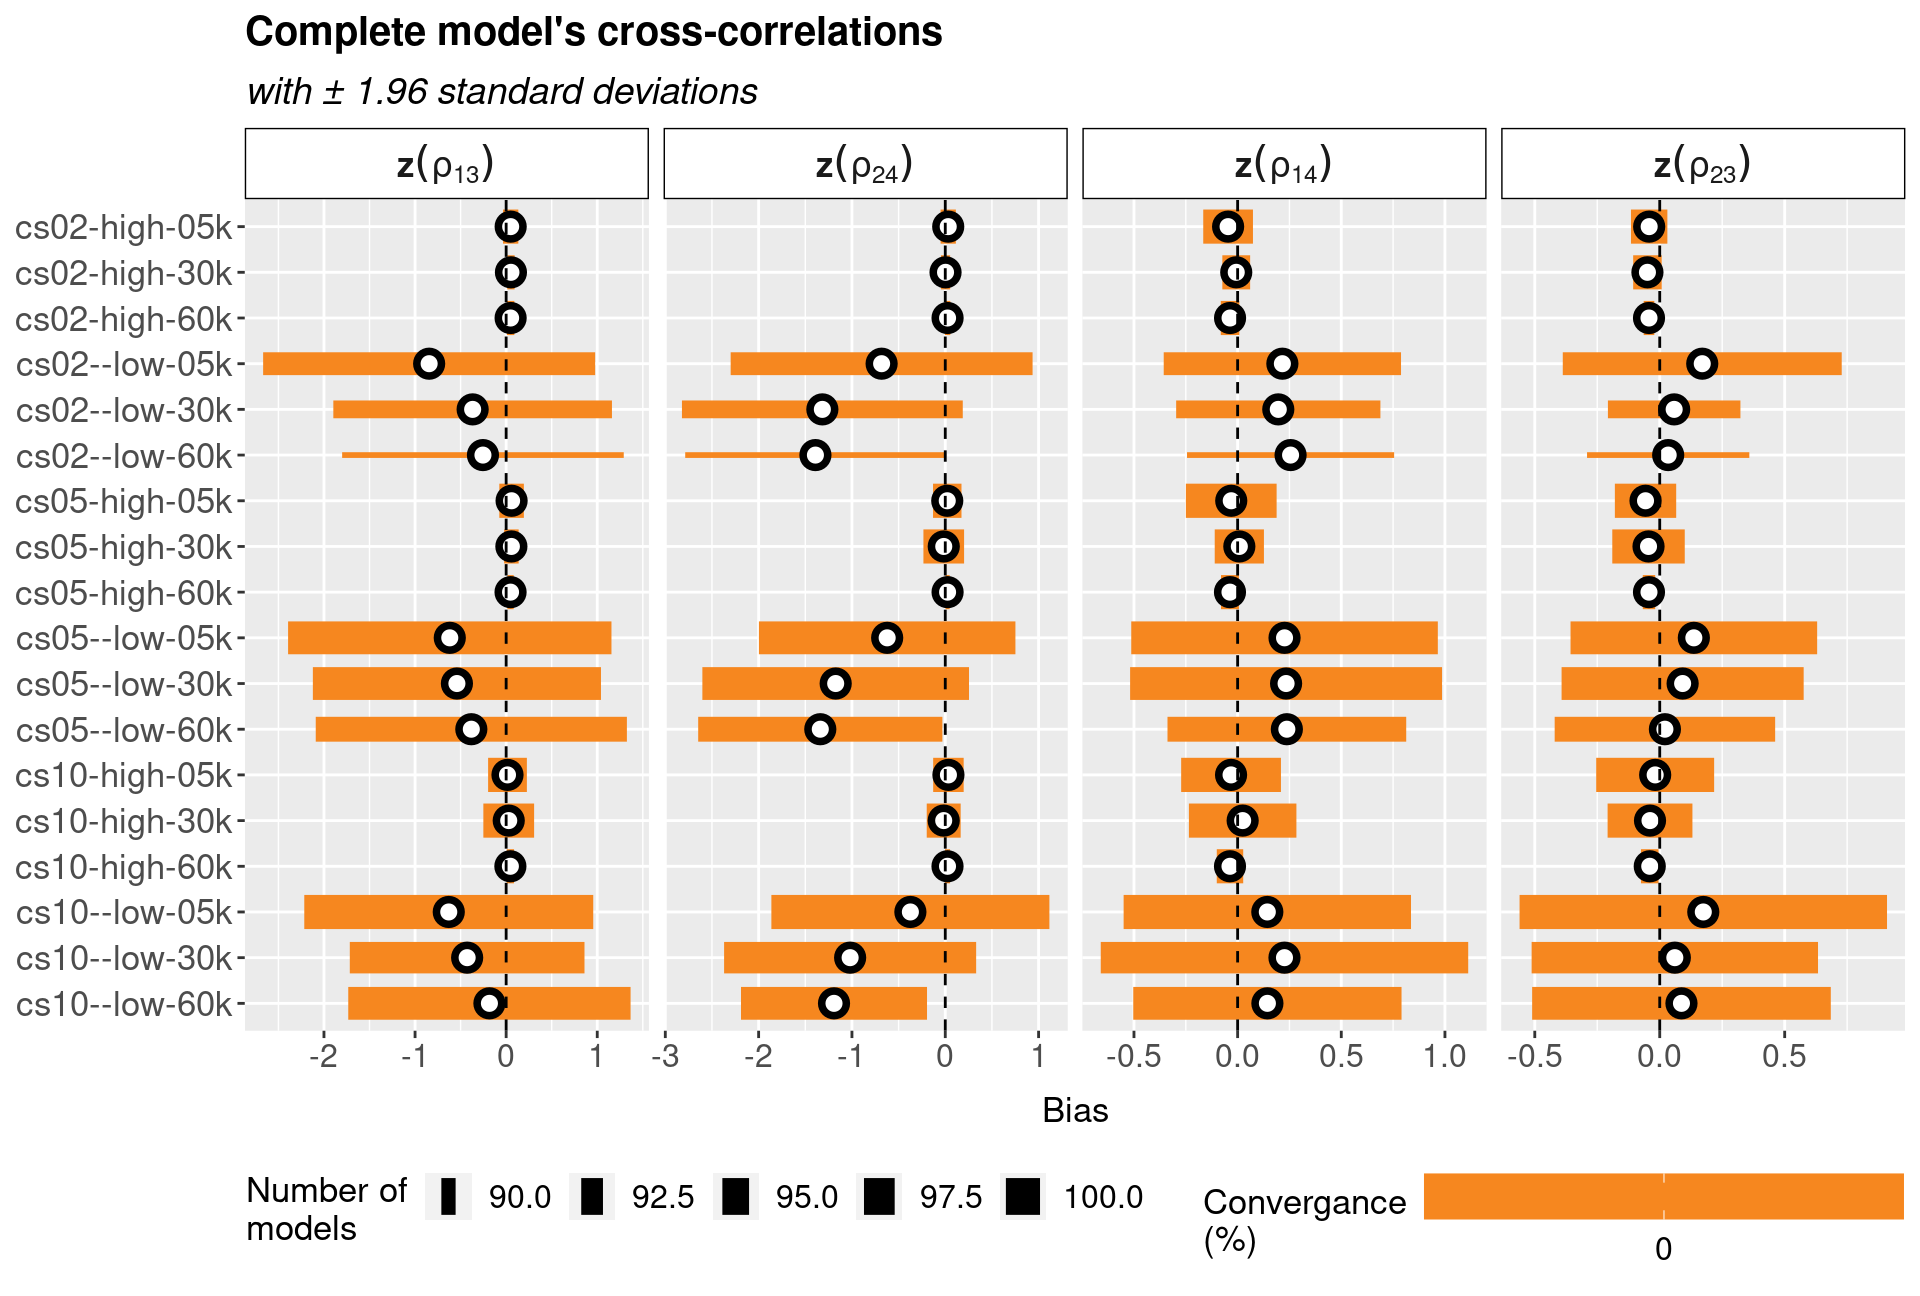
\includegraphics[width=\textwidth]{bias2plotsd-13.png}\\
 \begin{footnotesize}
  SOURCE: The author (2021).
 \end{footnotesize}
 \label{fig:biassdrhoz4}
\end{figure}

In each figure, we have the parameter bias and its uncertainty described
by a Wald-based interval i.e., \(\pm\) 1.96 the bias standard
deviation. The seventy-two scenarios are accommodated. We have up to
four blocks of bars, each one representing a model, and in each block,
we have eighteen bars each one representing the 300 fits in each of the
eighteen scenarios (\(4 \times 18 \times 300 = 21600\)). Each scenario
name consists of a combination of three strings. The cluster size (cs),
2, 5, and 10; the CIF configuration, high and low; the sample size, 5,
30, and 60 thousand. We tried to fit a total of 21600 models but not all
converged. Besides that inconvenience, the ones that converged do not
all converged in the strict sense of the word. To show these two
characteristics respectively, we control the bar widths and colors.

The ideal convergence is the traditional one i.e., based on the
gradient.

\begin{figure}[H]
 \setlength{\abovecaptionskip}{.0001pt}
 \caption{CUMULATIVE INCIDENCE FUNCTIONS (CIFs) HIGH}
 \vspace{0.2cm}\centering
 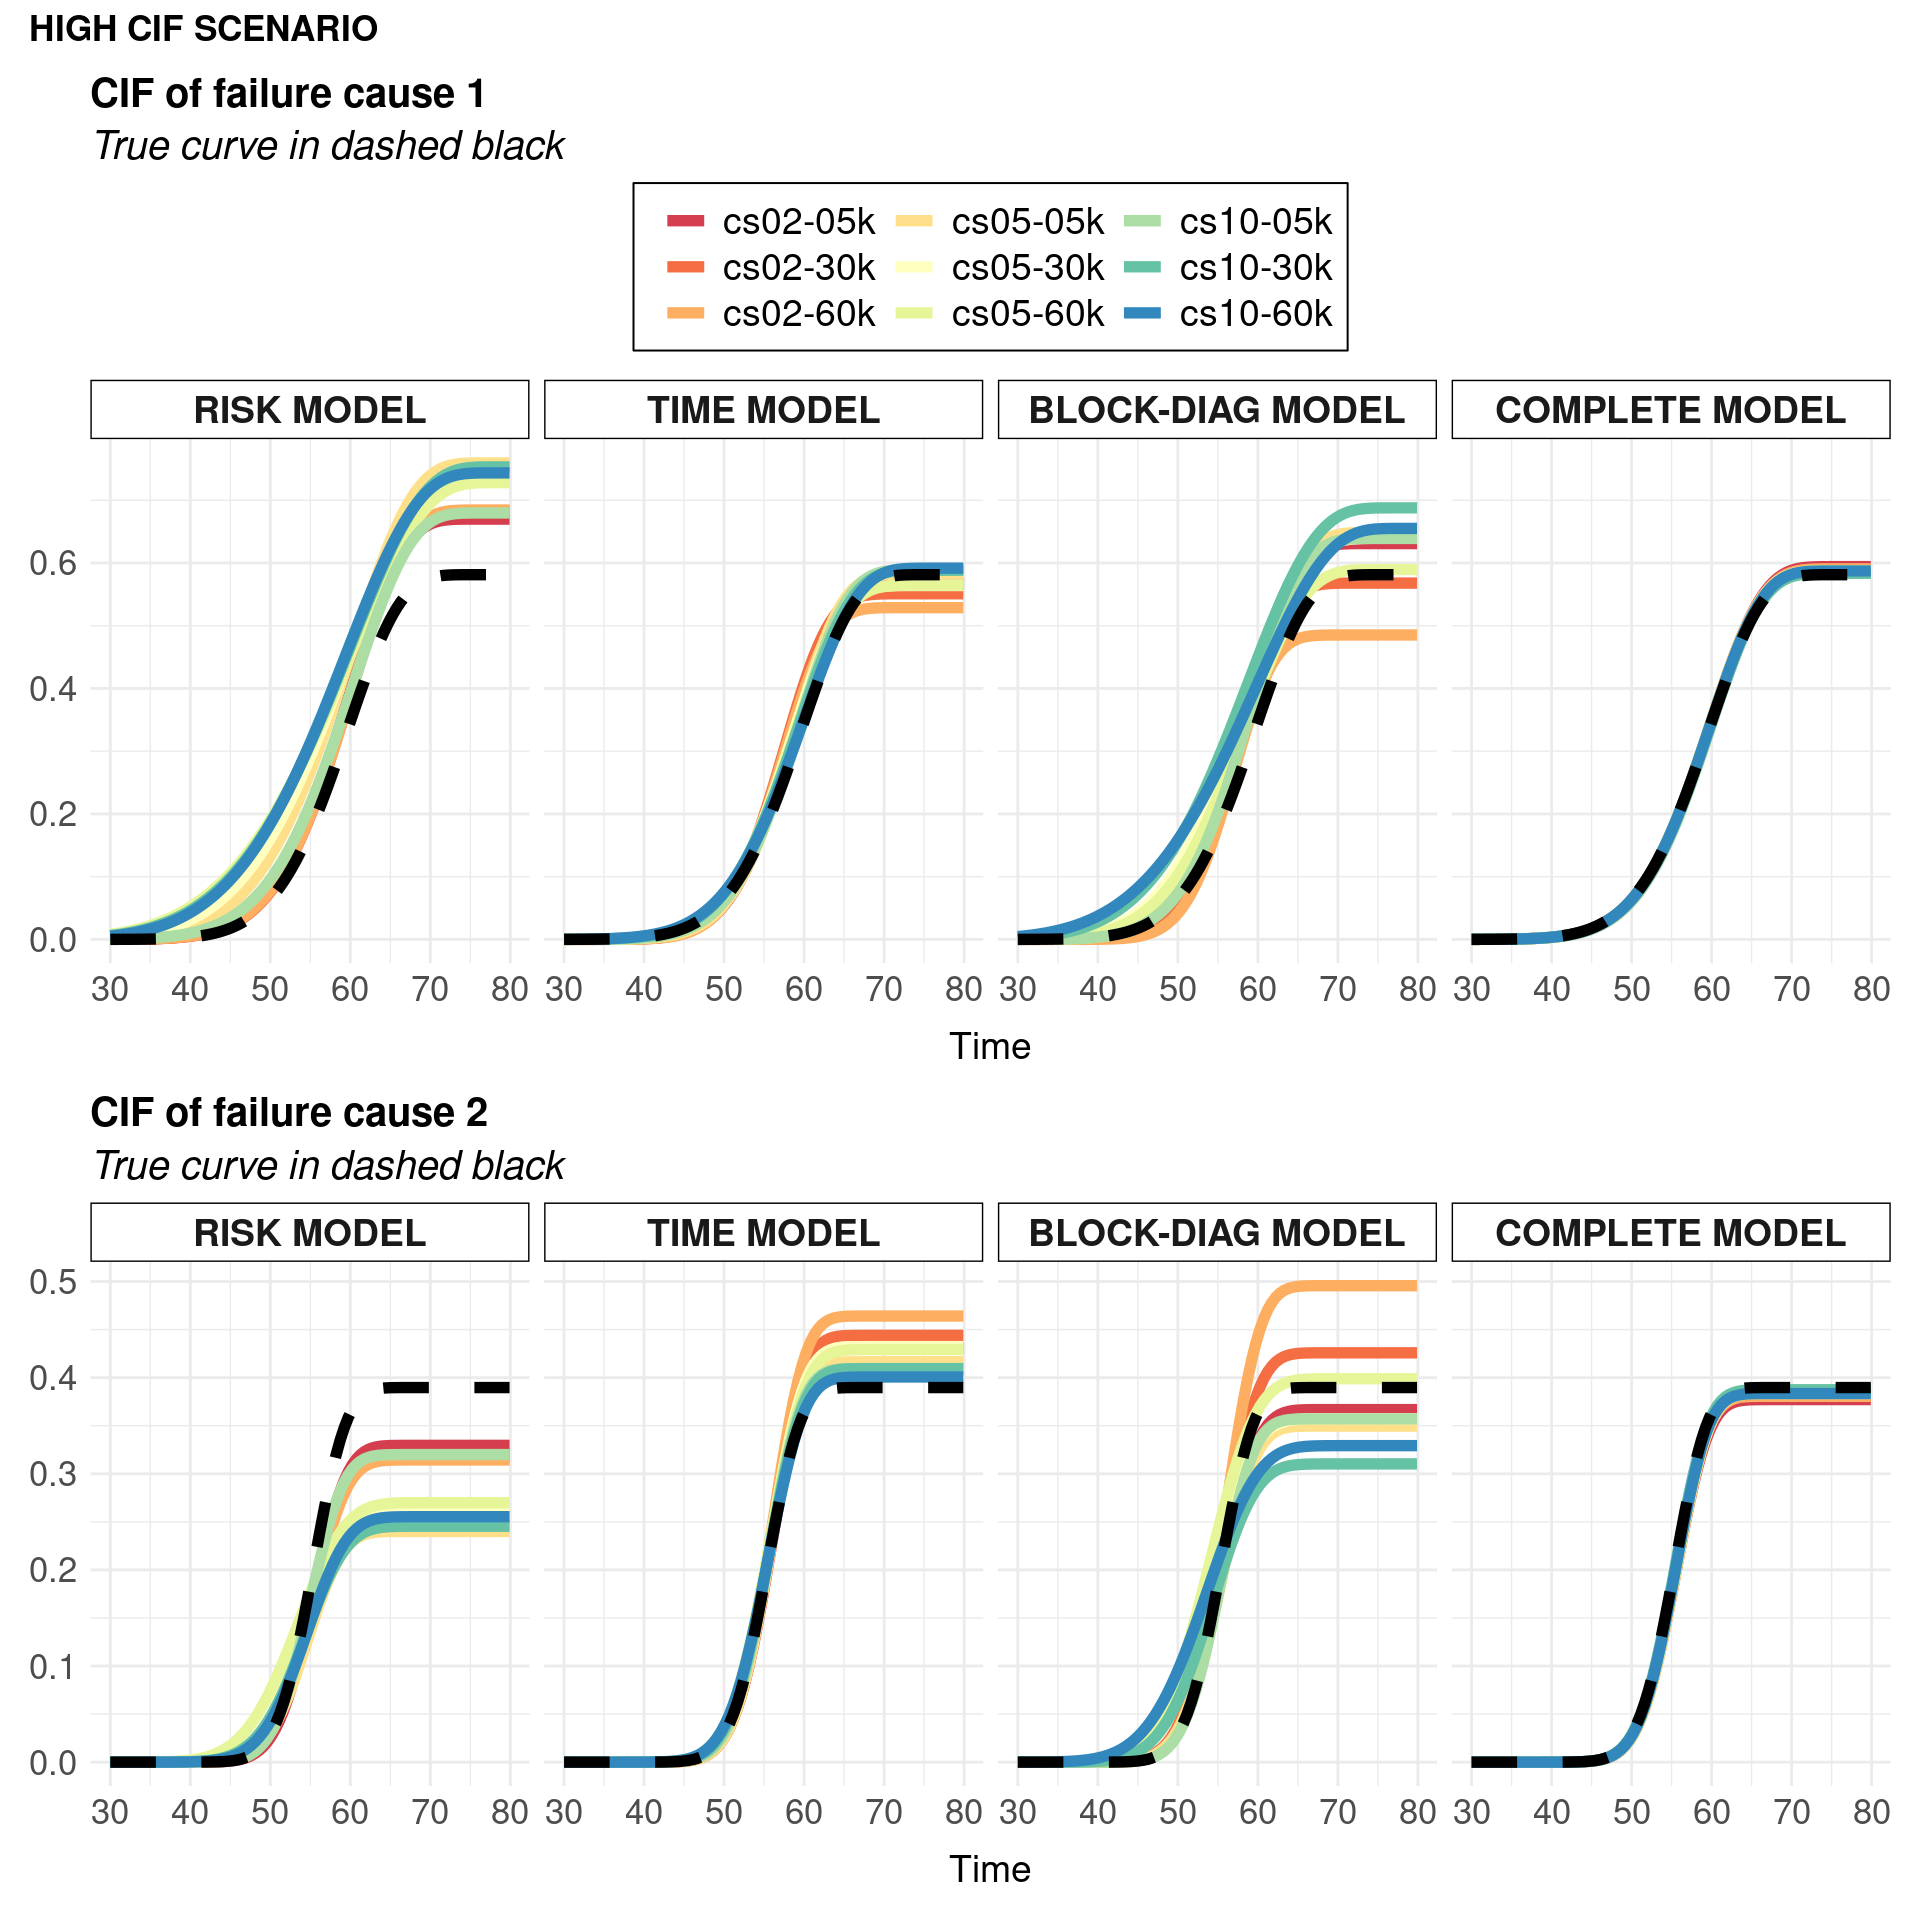
\includegraphics[width=\textwidth]{cifs-1.png}\\
 \begin{footnotesize}
  SOURCE: The author (2021).
 \end{footnotesize}
 \label{fig:cifshigh}
\end{figure}

\begin{figure}[H]
 \setlength{\abovecaptionskip}{.0001pt}
 \caption{CUMULATIVE INCIDENCE FUNCTIONS (CIFs) LOW}
 \vspace{0.2cm}\centering
 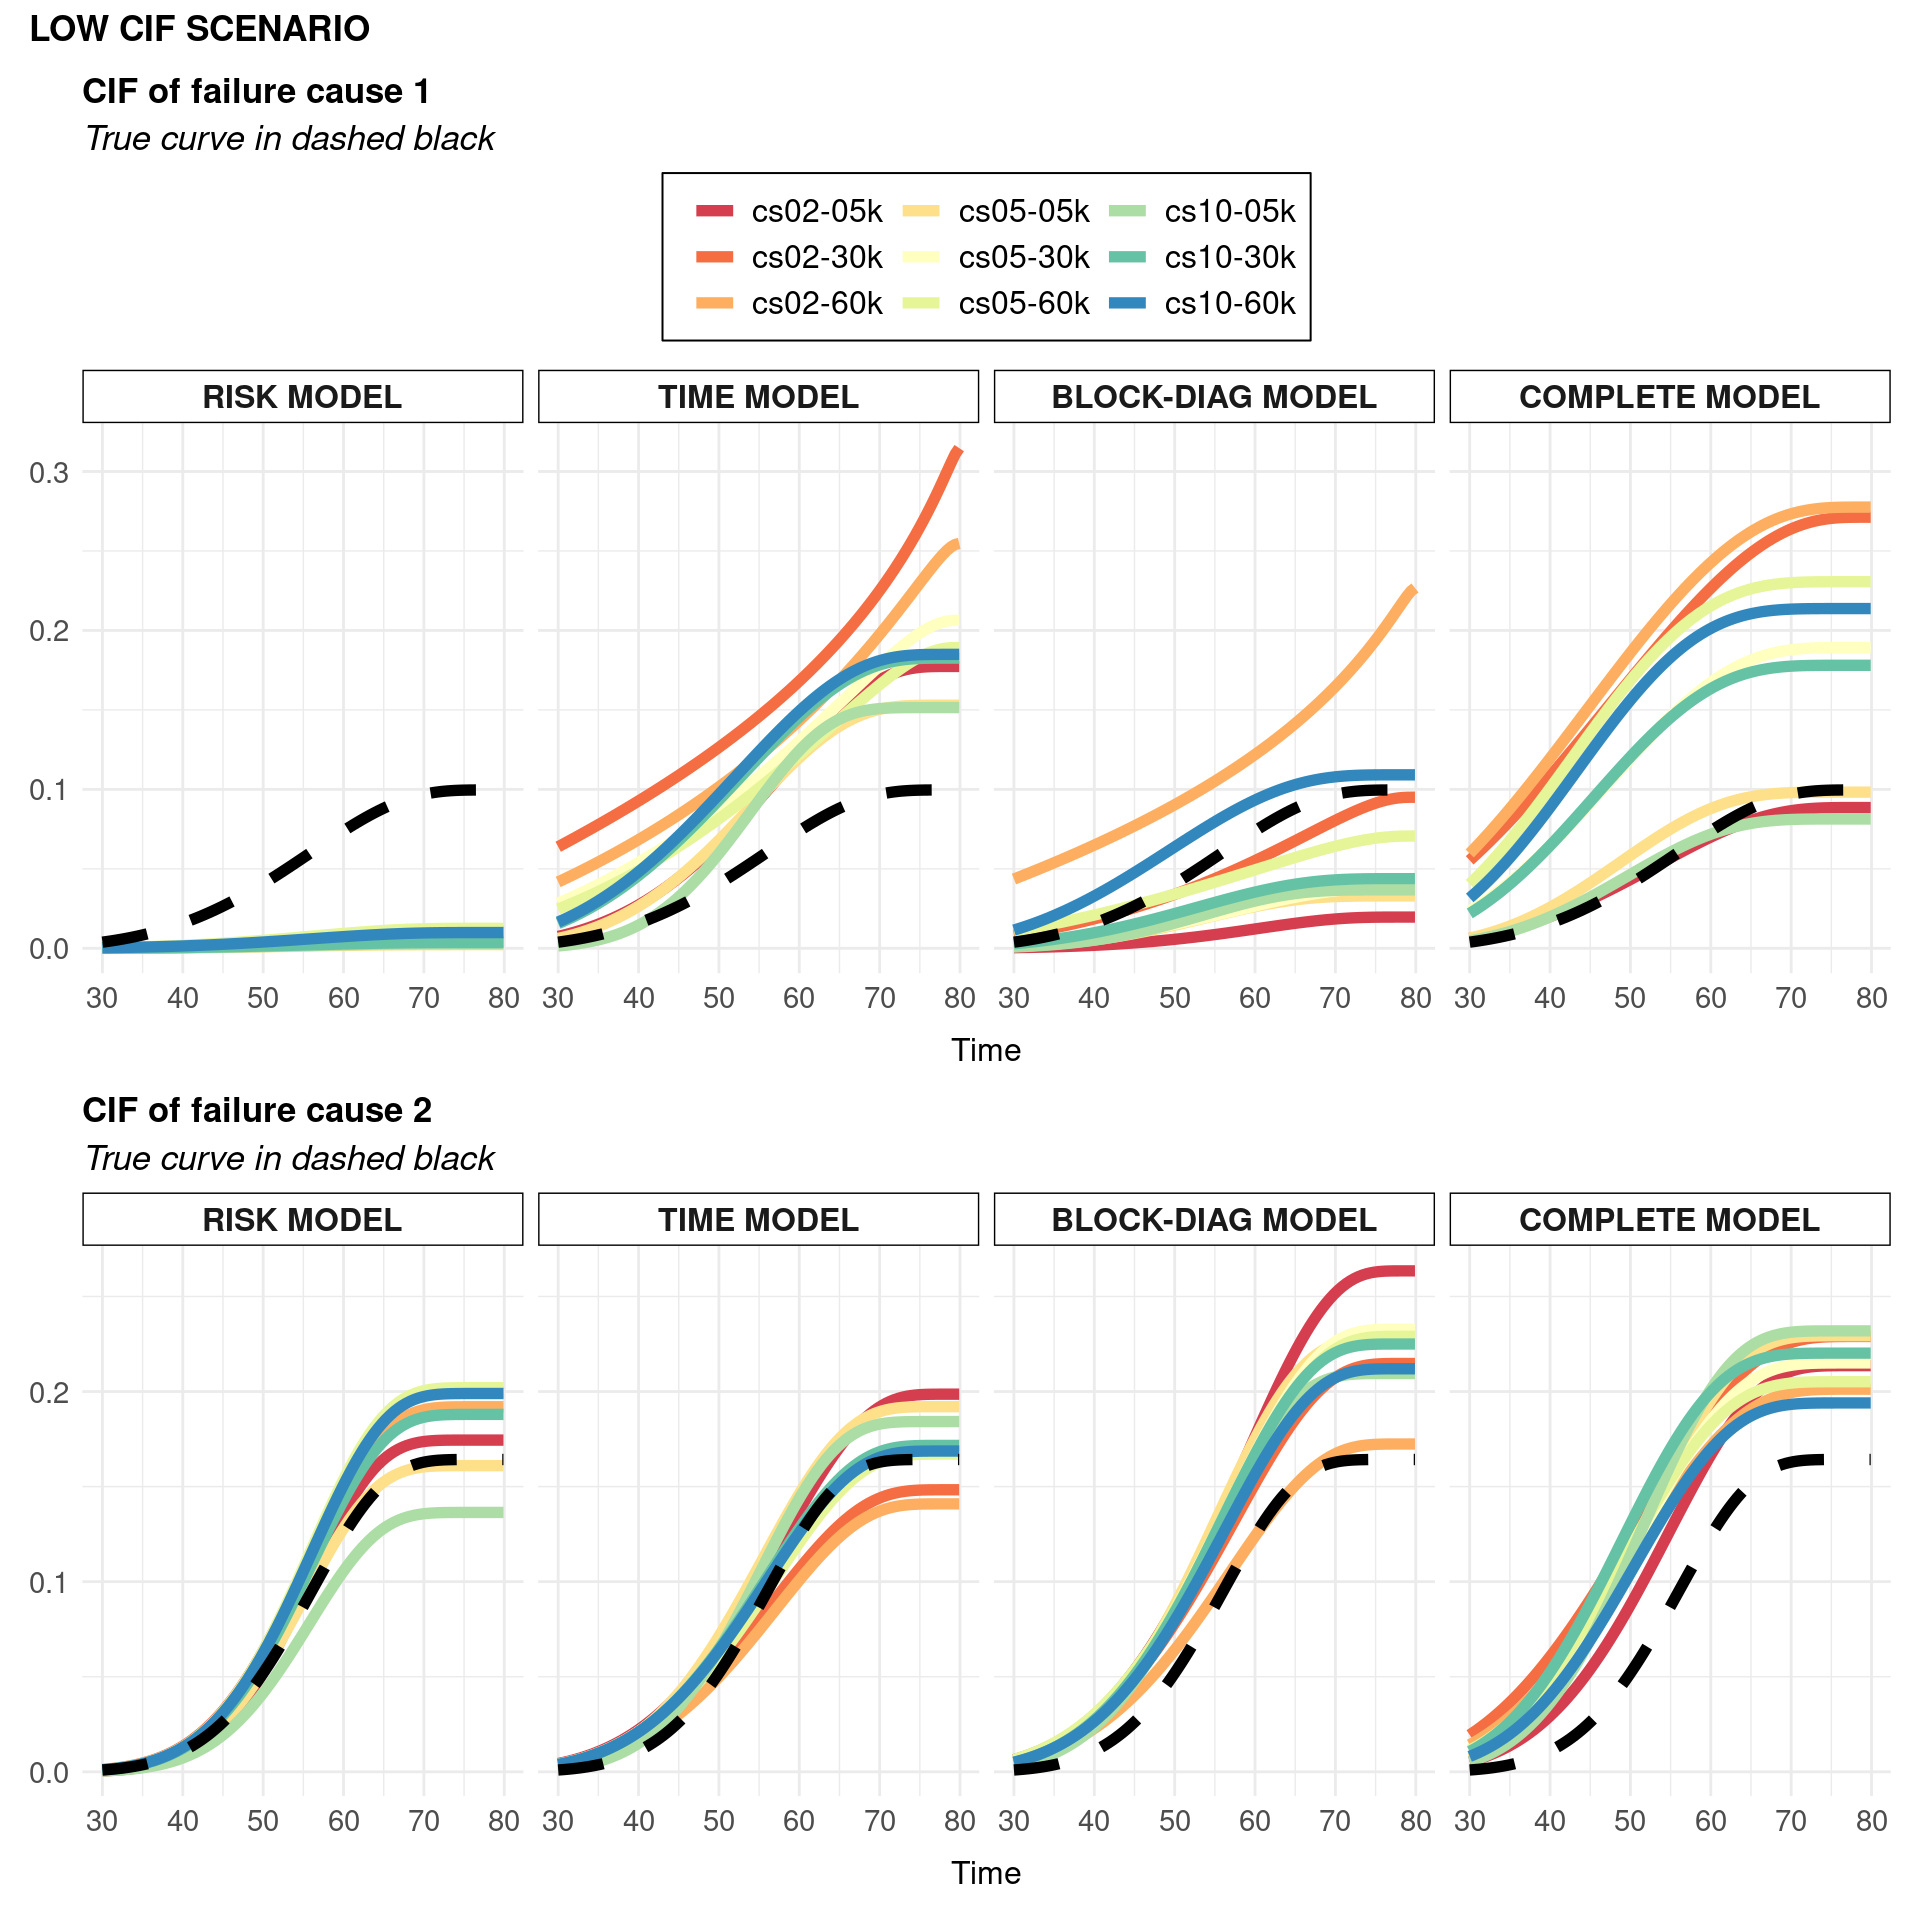
\includegraphics[width=\textwidth]{cifs-2.png}\\
 \begin{footnotesize}
  SOURCE: The author (2021).
 \end{footnotesize}
 \label{fig:cifslow}
\end{figure}

%% \begin{figure}[H]
%%  \setlength{\abovecaptionskip}{.0001pt}
%%  \caption{BUILDING \(\Sigma\)}
%%  \vspace{0.2cm}\centering
%%  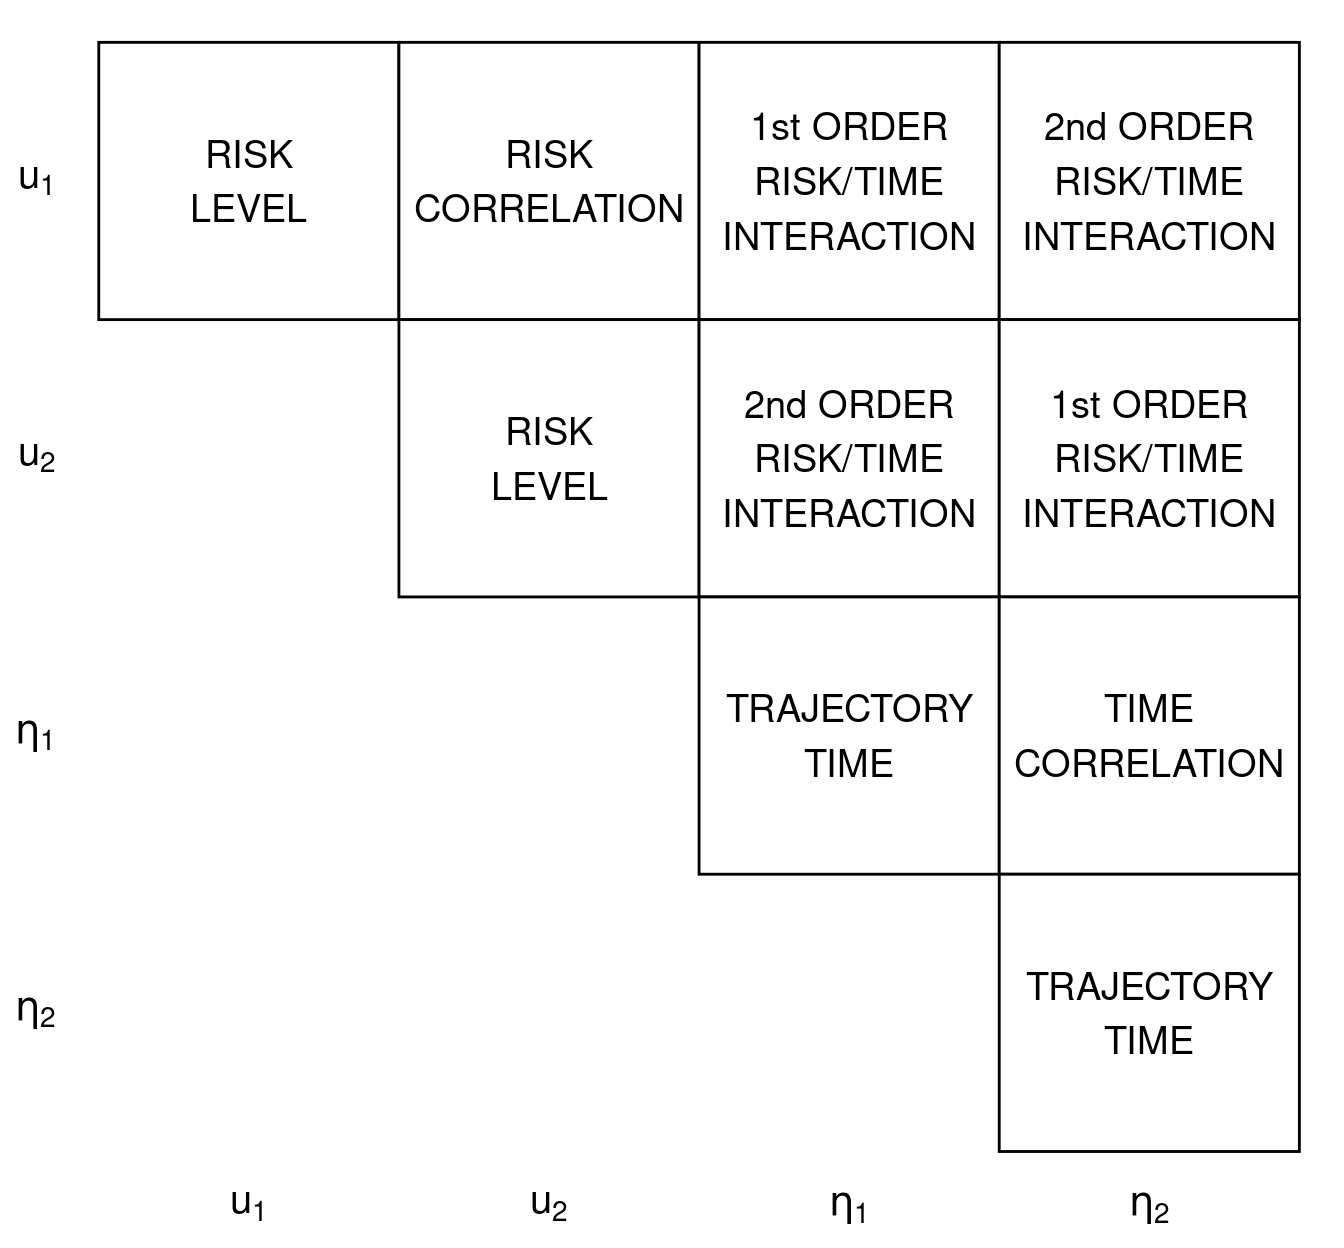
\includegraphics[width=0.75\textwidth]{buildingSigma-1.png}\\
%%  \begin{footnotesize}
%%   SOURCE: The author (2021).
%%  \end{footnotesize}
%%  \label{fig:buildingSigma}
%% \end{figure}

%% \begin{figure}[H]
%%  \setlength{\abovecaptionskip}{.0001pt}
%%  \caption{PARAMETERS CORRELATION}
%%  \vspace{0.2cm}\centering
%%  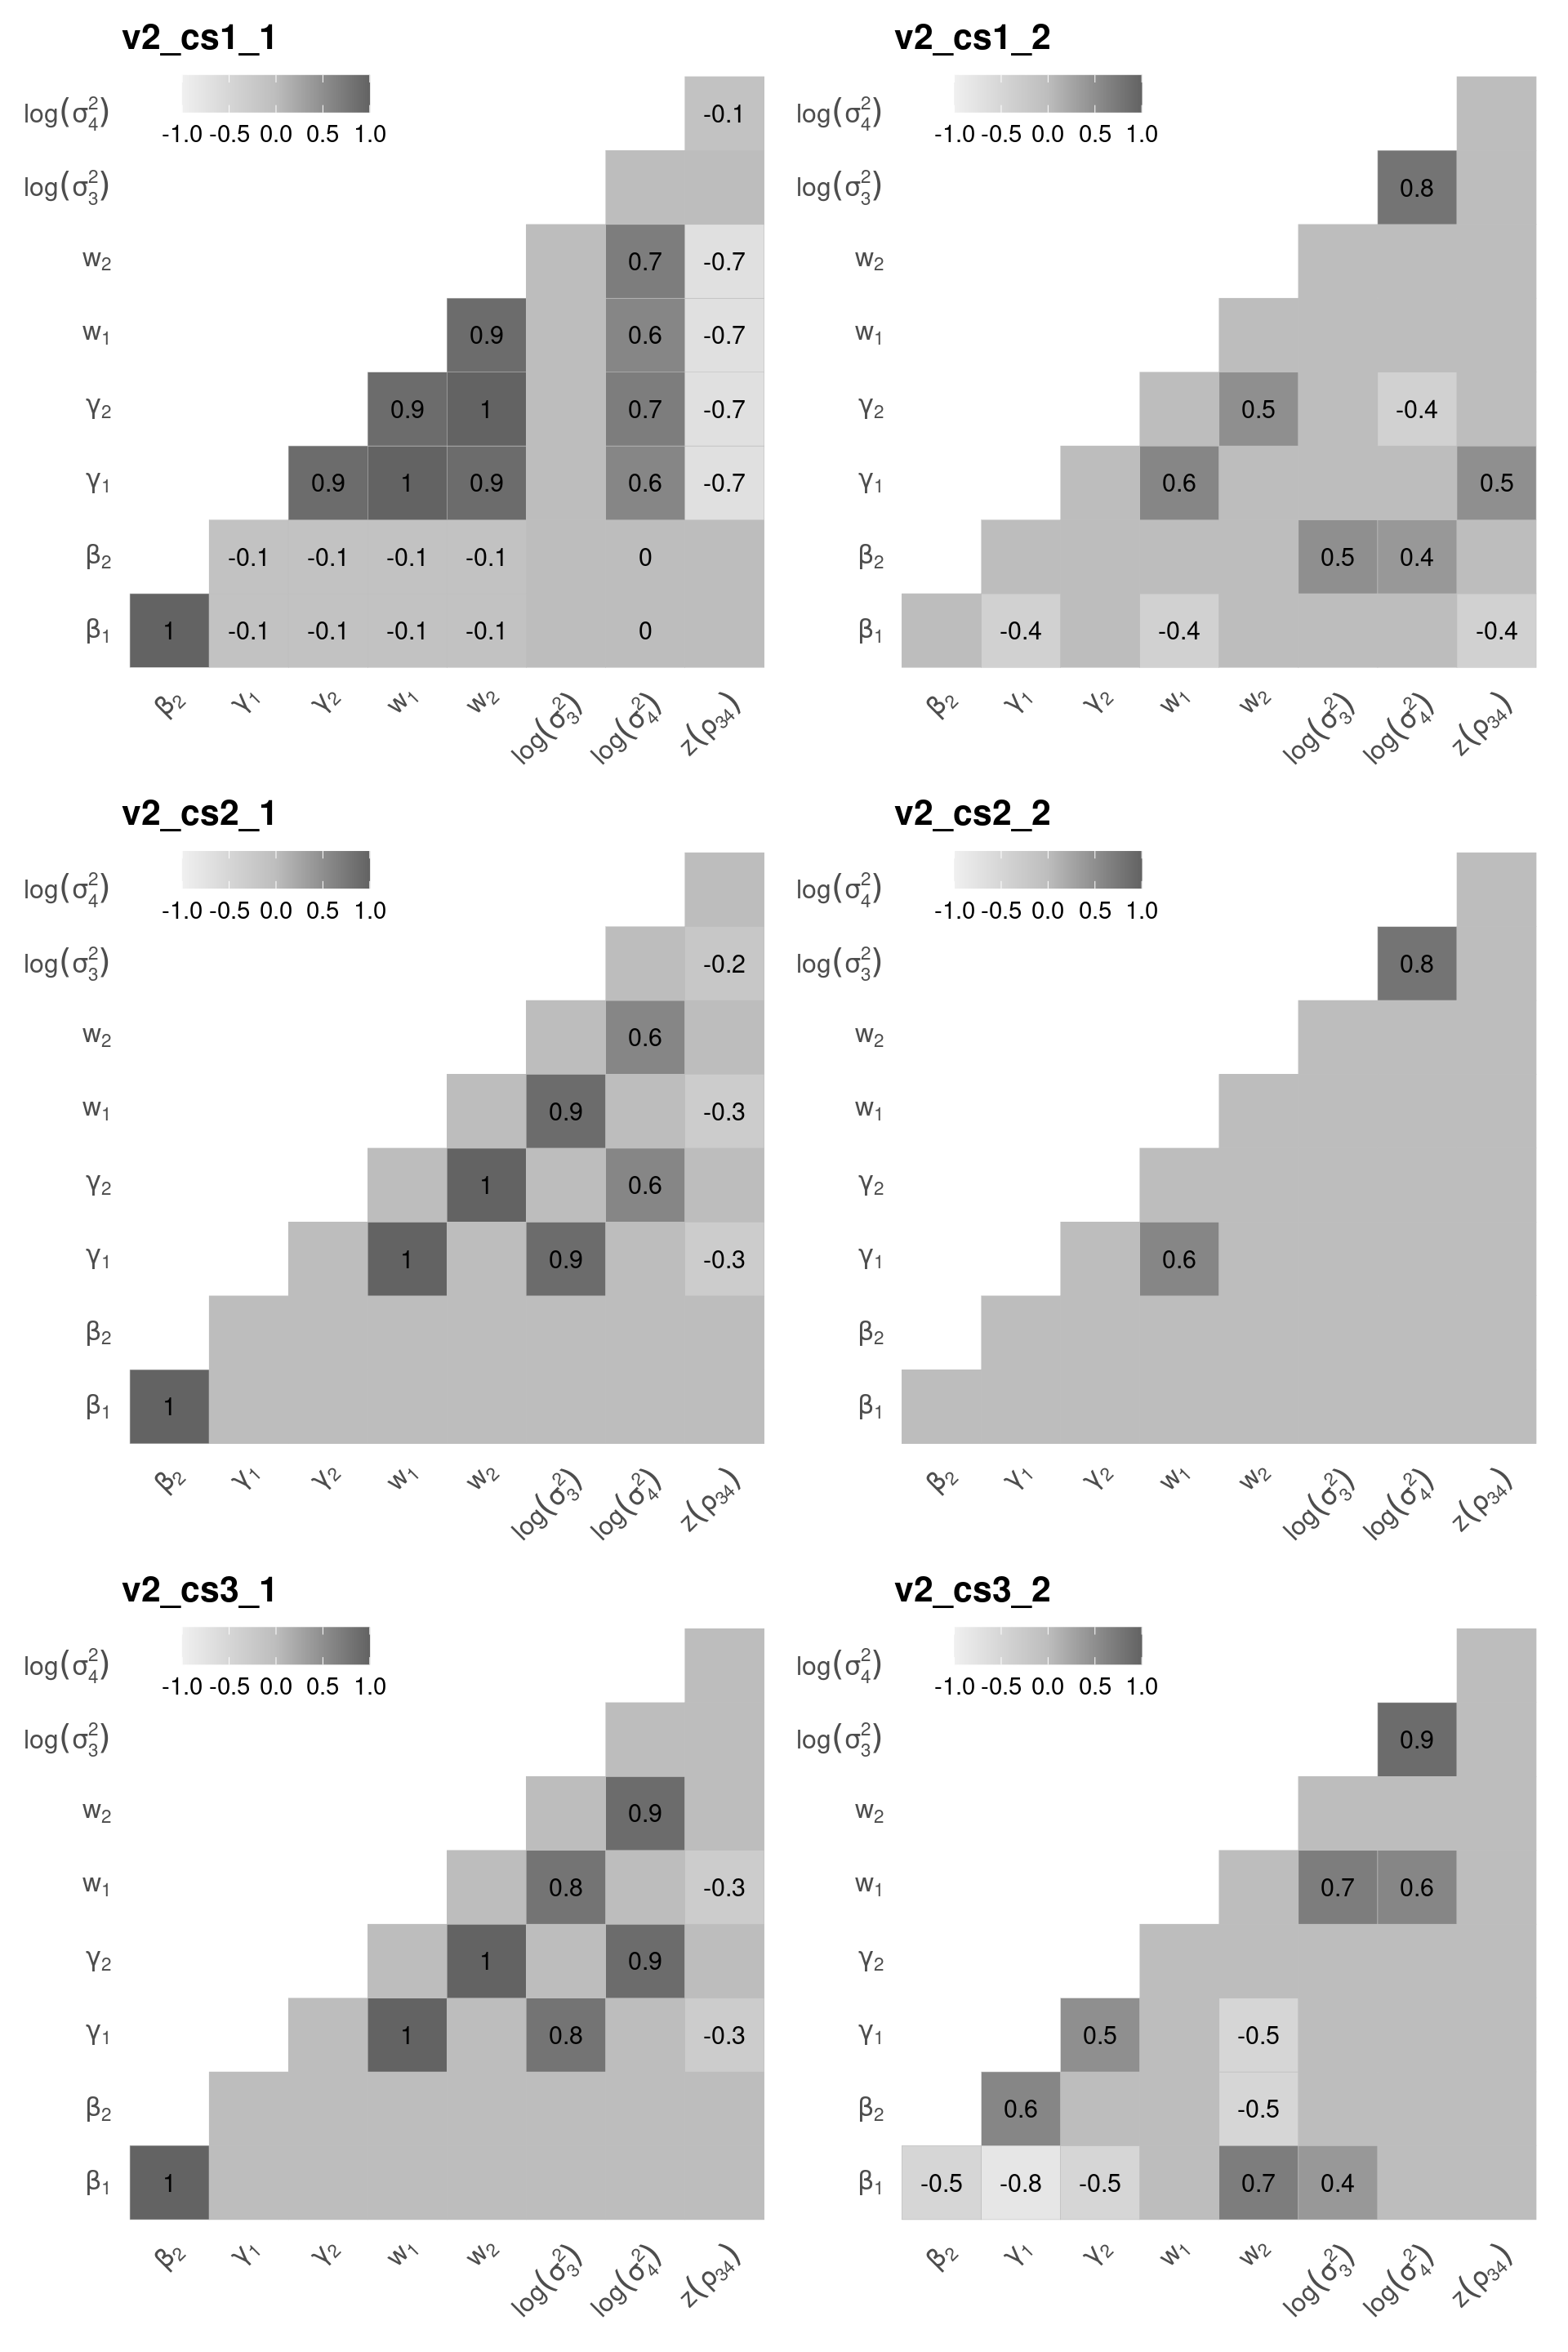
\includegraphics[width=\textwidth]{cor2plot-1.png}\\
%%  \begin{footnotesize}
%%   SOURCE: The author (2021).
%%  \end{footnotesize}
%%  \label{fig:cor2plot}
%% \end{figure}

%% \begin{figure}[H]
%%  \setlength{\abovecaptionskip}{.0001pt}
%%  \caption{VARIANCE-COVARIANCE MATRIX UPPER-TRIANGULAR COMPONENTS}
%%  \vspace{0.2cm}\centering
%%  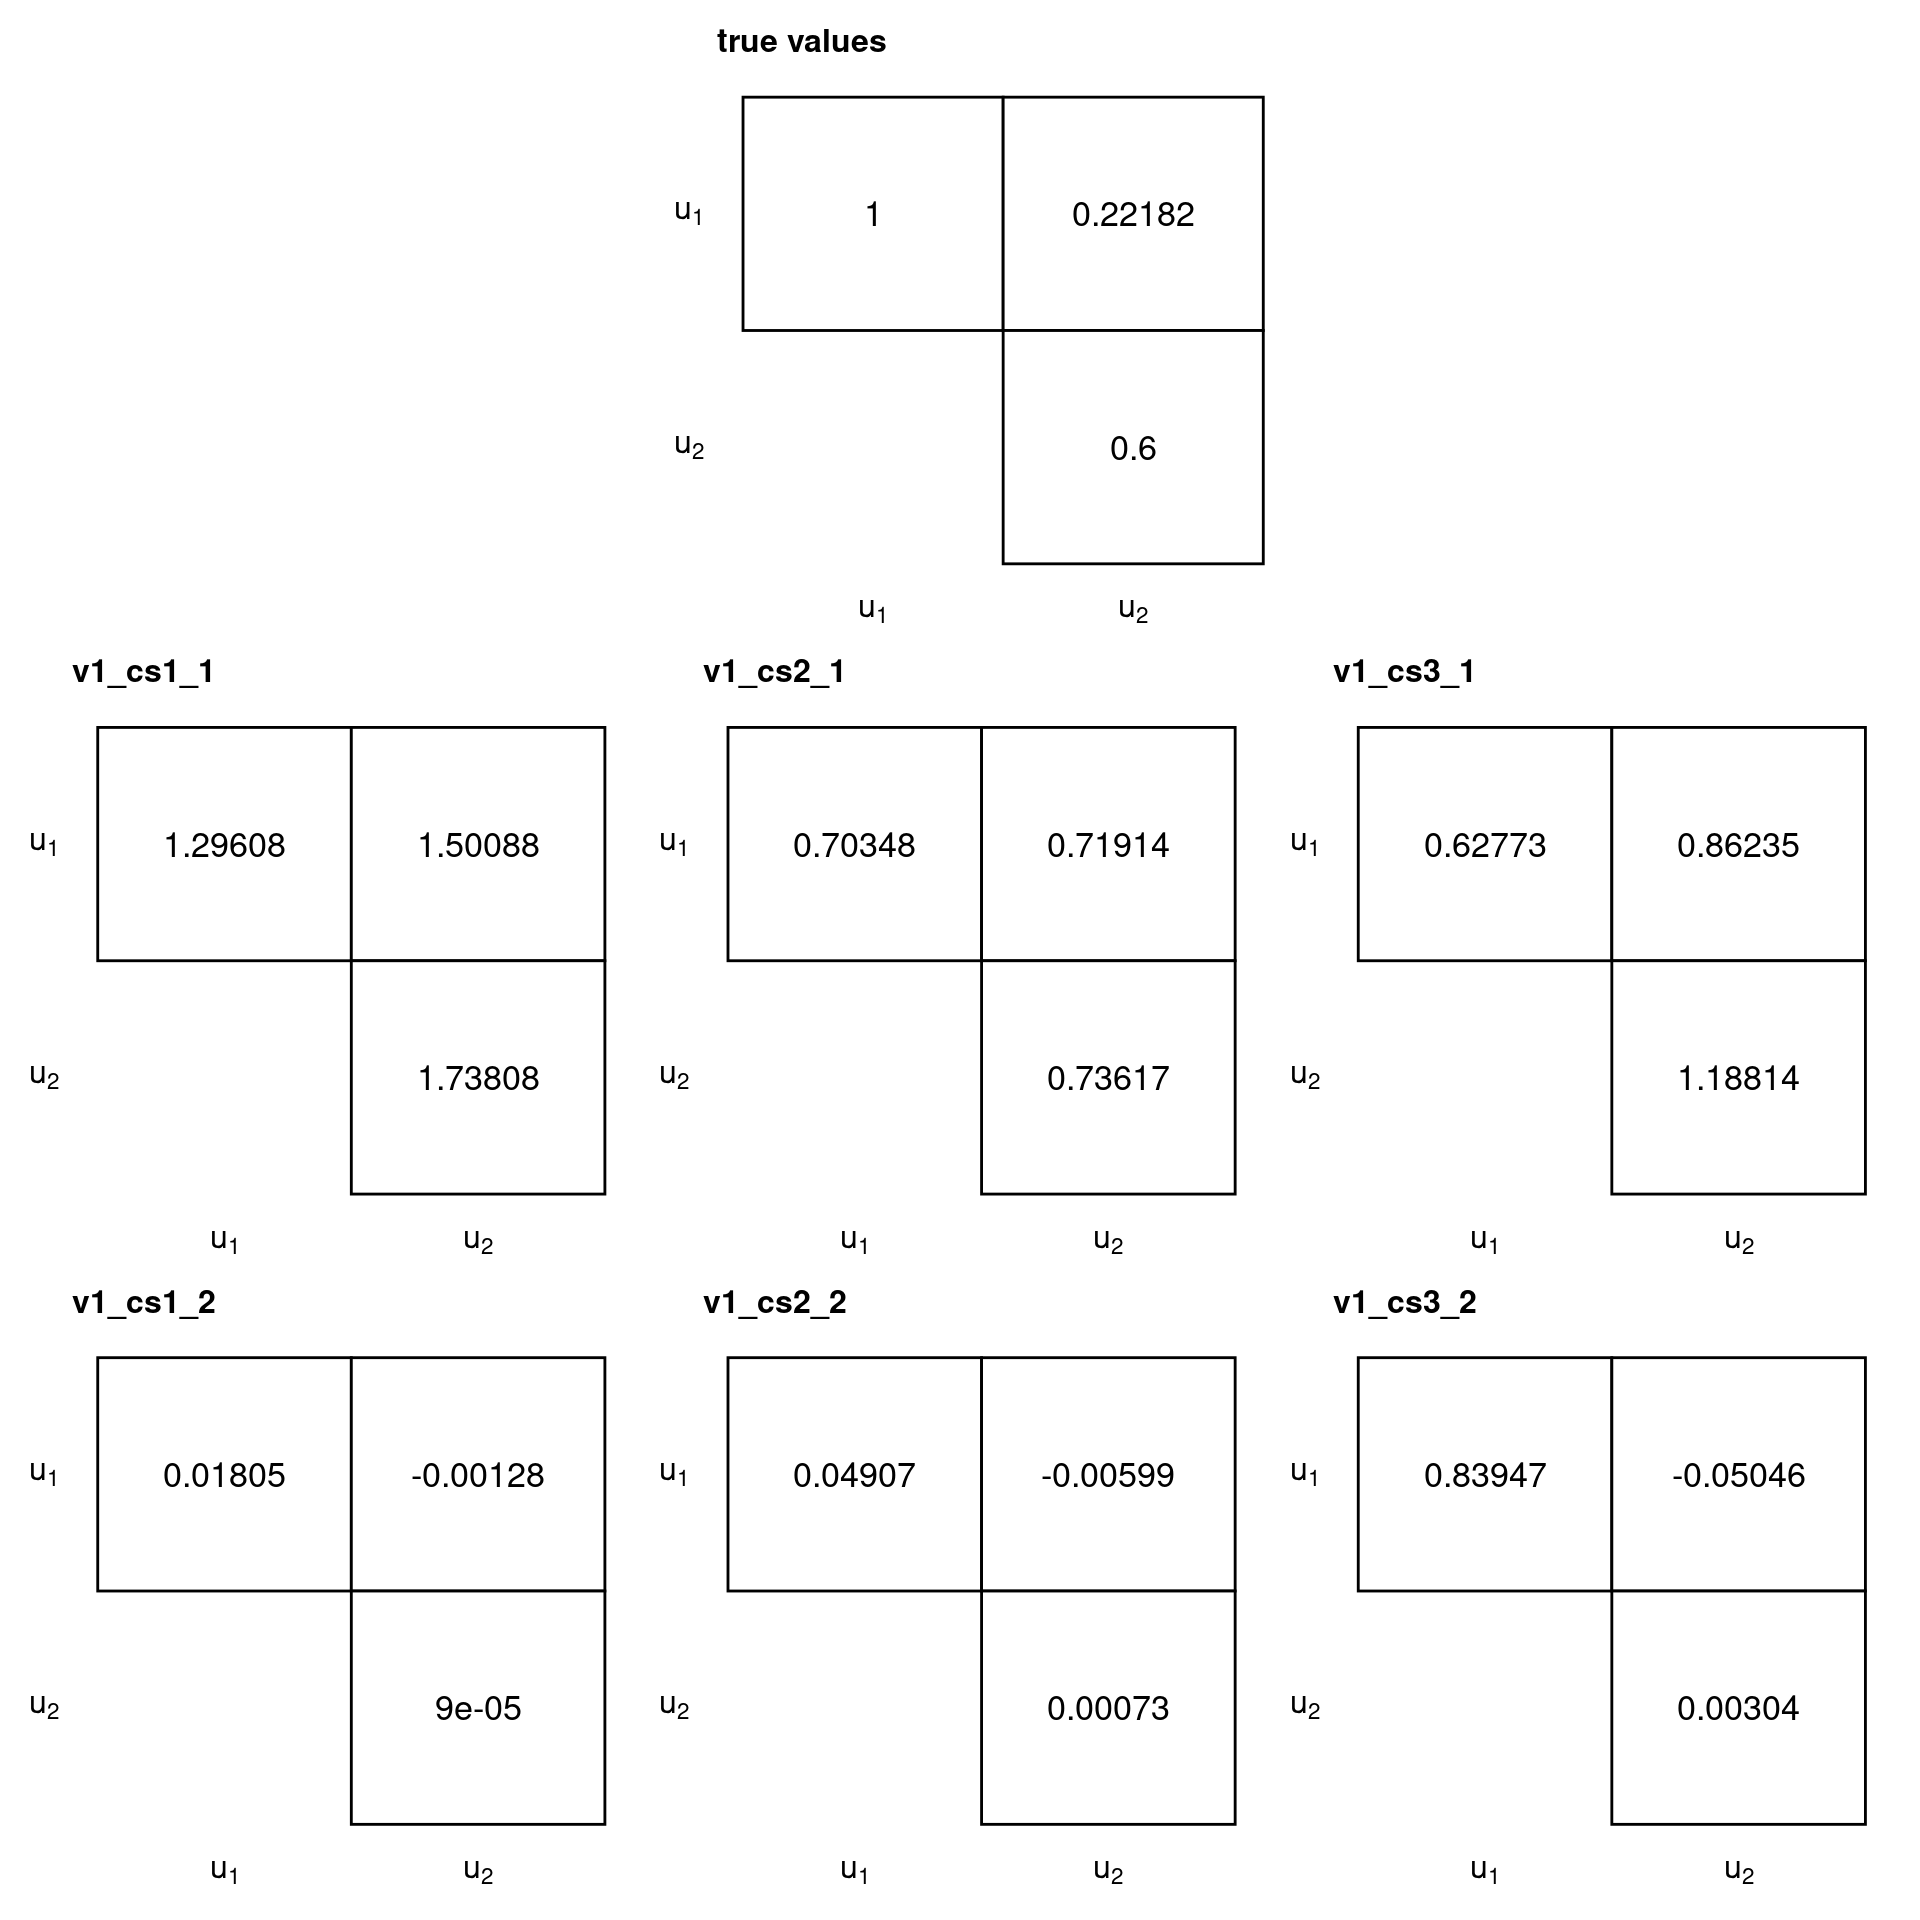
\includegraphics[width=\textwidth]{vcovs-1.png}\\
%%  \begin{footnotesize}
%%   SOURCE: The author (2021).
%%  \end{footnotesize}
%%  \label{fig:vcovs}
%% \end{figure}

% END ==================================================================
